%!TEX TS-program = xelatex

\documentclass[a4paper,14pt]{extarticle} % 14й шрифт
\usepackage[dvipsnames]{xcolor}
%%% Преамбула %%%

\usepackage{fontspec} % XeTeX
\usepackage{xunicode} % Unicode для XeTeX
\usepackage{xltxtra}  % Верхние и нижние индексы
\usepackage{pdfpages} % Вставка PDF

\usepackage{listings} % Оформление исходного кода
\lstset{
    basicstyle=\small\ttfamily, % Размер и тип шрифта
    breaklines=true, % Перенос строк
    tabsize=2, % Размер табуляции
    literate={--}{{-{}-}}2 % Корректно отображать двойной дефис
}

% Шрифты, xelatex
\defaultfontfeatures{Ligatures=TeX}
\setmainfont{Times New Roman} % Нормоконтроллеры хотят именно его
\newfontfamily{\cyrillicfonttt}{Times New Roman}
%\setsansfont{Liberation Sans} % Тут я его не использую, но если пригодится
\setmonofont{Consolas} % Моноширинный шрифт для оформления кода


% Русский язык
\usepackage{polyglossia}
\setdefaultlanguage{russian}

\usepackage{amssymb,amsfonts,amsmath} % Математика
\numberwithin{equation}{section} % Формула вида секция.номер

\usepackage{enumerate} % Тонкая настройка списков
\usepackage{indentfirst} % Красная строка после заголовка
\usepackage{float} % Расширенное управление плавающими объектами
\usepackage{multirow} % Сложные таблицы

% Пути к каталогам с изображениями
\usepackage{graphicx} % Вставка картинок и дополнений
\graphicspath{{images/}{images/userguide/}{images/testing/}{images/infrastructure/}{extra/}{extra/drafts/}}

% Формат подрисуночных записей
\usepackage{chngcntr}
\counterwithout{figure}{section}

% Гиперссылки
\usepackage{hyperref}
\hypersetup{
    colorlinks, urlcolor={black}, % Все ссылки черного цвета, кликабельные
    linkcolor={black}, citecolor={black}, filecolor={black},
    pdfauthor={Глеб Щенников},
    pdftitle={Плагин захвата мимики}
}

% Оформление библиографии и подрисуночных записей через точку
\makeatletter
\renewcommand*{\@biblabel}[1]{\hfill#1.}
\renewcommand*\l@section{\@dottedtocline{1}{1em}{1em}}
\renewcommand{\thefigure}{\arabic{figure}} % Формат рисунка секция.номер
\renewcommand{\thetable}{\thesection.\arabic{table}} % Формат таблицы секция.номер
\def\redeflsection{\def\l@section{\@dottedtocline{1}{0em}{10em}}}
\makeatother

\renewcommand{\baselinestretch}{1.4} % Полуторный межстрочный интервал
\parindent 1.27cm % Абзацный отступ

\sloppy             % Избавляемся от переполнений
\hyphenpenalty=1000 % Частота переносов
\clubpenalty=10000  % Запрещаем разрыв страницы после первой строки абзаца
\widowpenalty=10000 % Запрещаем разрыв страницы после последней строки абзаца

% Отступы у страниц
\usepackage{geometry}
\geometry{left=3cm}
\geometry{right=1.5cm}
\geometry{top=2cm}
\geometry{bottom=2cm}

% Списки
\usepackage{enumitem}
\setlist[enumerate,itemize]{leftmargin=12.7mm} % Отступы в списках

\makeatletter
    \AddEnumerateCounter{\asbuk}{\@asbuk}{м)}
\makeatother
\setlist{nolistsep} % Нет отступов между пунктами списка
\renewcommand{\labelitemi}{--} % Маркет списка --
\renewcommand{\labelenumi}{\asbuk{enumi})} % Список второго уровня
\renewcommand{\labelenumii}{\arabic{enumii})} % Список третьего уровня

% Содержание
\usepackage{tocloft}
\renewcommand{\cfttoctitlefont}{\hspace{0.38\textwidth}\MakeTextUppercase} % СОДЕРЖАНИЕ
\renewcommand{\cftsecfont}{\hspace{0pt}}            % Имена секций в содержании не жирным шрифтом
\renewcommand\cftsecleader{\cftdotfill{\cftdotsep}} % Точки для секций в содержании
\renewcommand\cftsecpagefont{\mdseries}             % Номера страниц не жирные
\setcounter{tocdepth}{3}                            % Глубина оглавления, до subsubsection

% Нумерация страниц по центру снизу
\usepackage{fancyhdr}
\pagestyle{fancy}
\fancyhf{}
\fancyfoot[C]{\thepage} % Page numbering for center header  
\fancyheadoffset{0mm}
\fancyfootoffset{0mm}
\setlength{\headheight}{17pt}
\renewcommand{\headrulewidth}{0pt}
\renewcommand{\footrulewidth}{0pt}
\fancypagestyle{plain}{ 
    \fancyhf{}
    \rhead{\thepage}
}

%таблицы помещаются в страницу
\usepackage{adjustbox}

% Формат подрисуночных надписей
\RequirePackage{caption}
\DeclareCaptionLabelSeparator{defffis}{ -- } % Разделитель
\captionsetup[figure]{justification=centering, labelsep=defffis, format=plain} % Подпись рисунка по центру
\captionsetup[table]{justification=raggedright, labelsep=defffis, format=plain, singlelinecheck=false} % Подпись таблицы слева
\addto\captionsrussian{\renewcommand{\figurename}{Рисунок}} % Имя фигуры

% Пользовательские функции
\newcommand{\addimg}[4]{ % Добавление одного рисунка
    \begin{figure}
        \centering
        \includegraphics[width=#2\linewidth]{#1}
        \caption{#3} \label{#4}
    \end{figure}
}
\newcommand{\addimghere}[4]{ % Добавить рисунок непосредственно в это место
    \begin{figure}[H]
        \centering
        \includegraphics[width=#2\linewidth]{#1}
        \caption{#3} \label{#4}
    \end{figure}
}
\newcommand{\addtwoimghere}[5]{ % Вставка двух рисунков
    \begin{figure}[H]
        \centering
        \includegraphics[width=#2\linewidth]{#1}
        \hfill
        \includegraphics[width=#3\linewidth]{#2}
        \caption{#4} \label{#5}
    \end{figure}
}
\newcommand{\addimgapp}[2]{ % Это костыль для приложения Б
    \begin{figure}[H]
        \centering
        \includegraphics[width=1\linewidth]{#1}
        \caption*{#2}
    \end{figure}
}

% Заголовки секций в оглавлении в верхнем регистре
\usepackage{textcase}
\makeatletter
\let\oldcontentsline\contentsline
\def\contentsline#1#2{
    \expandafter\ifx\csname l@#1\endcsname\l@section
        \expandafter\@firstoftwo
    \else
        \expandafter\@secondoftwo
    \fi
    {\oldcontentsline{#1}{\MakeTextUppercase{#2}}}
    {\oldcontentsline{#1}{#2}}
}
\makeatother

% Оформление заголовков
\usepackage[compact,explicit]{titlesec}
\titleformat{\section}{}{}{12.5mm}{\bfseries{\thesection\quad#1}\vspace{0.5em}}
\titleformat{\subsection}[block]{\bfseries\vspace{1em}}{}{12.5mm}{\thesubsection\quad#1\vspace{0.5em}}
\titleformat{\subsubsection}[block]{\bfseries\vspace{1em}\normalsize}{}{12.5mm}{\thesubsubsection\quad#1\vspace{0.5em}}
\titleformat{\paragraph}[block]{\bfseries\normalsize}{}{12.5mm}{\MakeTextUppercase{#1}}

% Секции без номеров (введение, заключение...), вместо section*{}
\newcommand{\anonsection}[1]{
    \phantomsection % Корректный переход по ссылкам в содержании
    \paragraph{\centerline{{#1}}\vspace{1.5em}}
    \addcontentsline{toc}{section}{\uppercase{#1}}
}

% Секции для приложений
\newcommand{\appsection}[1]{
    \phantomsection
    \paragraph{\centerline{{#1}}}
    \addcontentsline{toc}{section}{\uppercase{#1}}
}

% Библиография: отступы и межстрочный интервал
\makeatletter
\renewenvironment{thebibliography}[1]
    {\section*{\refname}
        \list{\@biblabel{\@arabic\c@enumiv}}
           {\settowidth\labelwidth{\@biblabel{#1}}
            \leftmargin\labelsep
            \itemindent 16.7mm
            \@openbib@code
            \usecounter{enumiv}
            \let\p@enumiv\@empty
            \renewcommand\theenumiv{\@arabic\c@enumiv}
        }
        \setlength{\itemsep}{0pt}
    }
\makeatother

\setcounter{page}{3} % Начало нумерации страниц
 % Подключаем преамбулу

%%% Начало документа
\begin{document}

%
\includepdf{otchpr} % Индивидуальное задание
%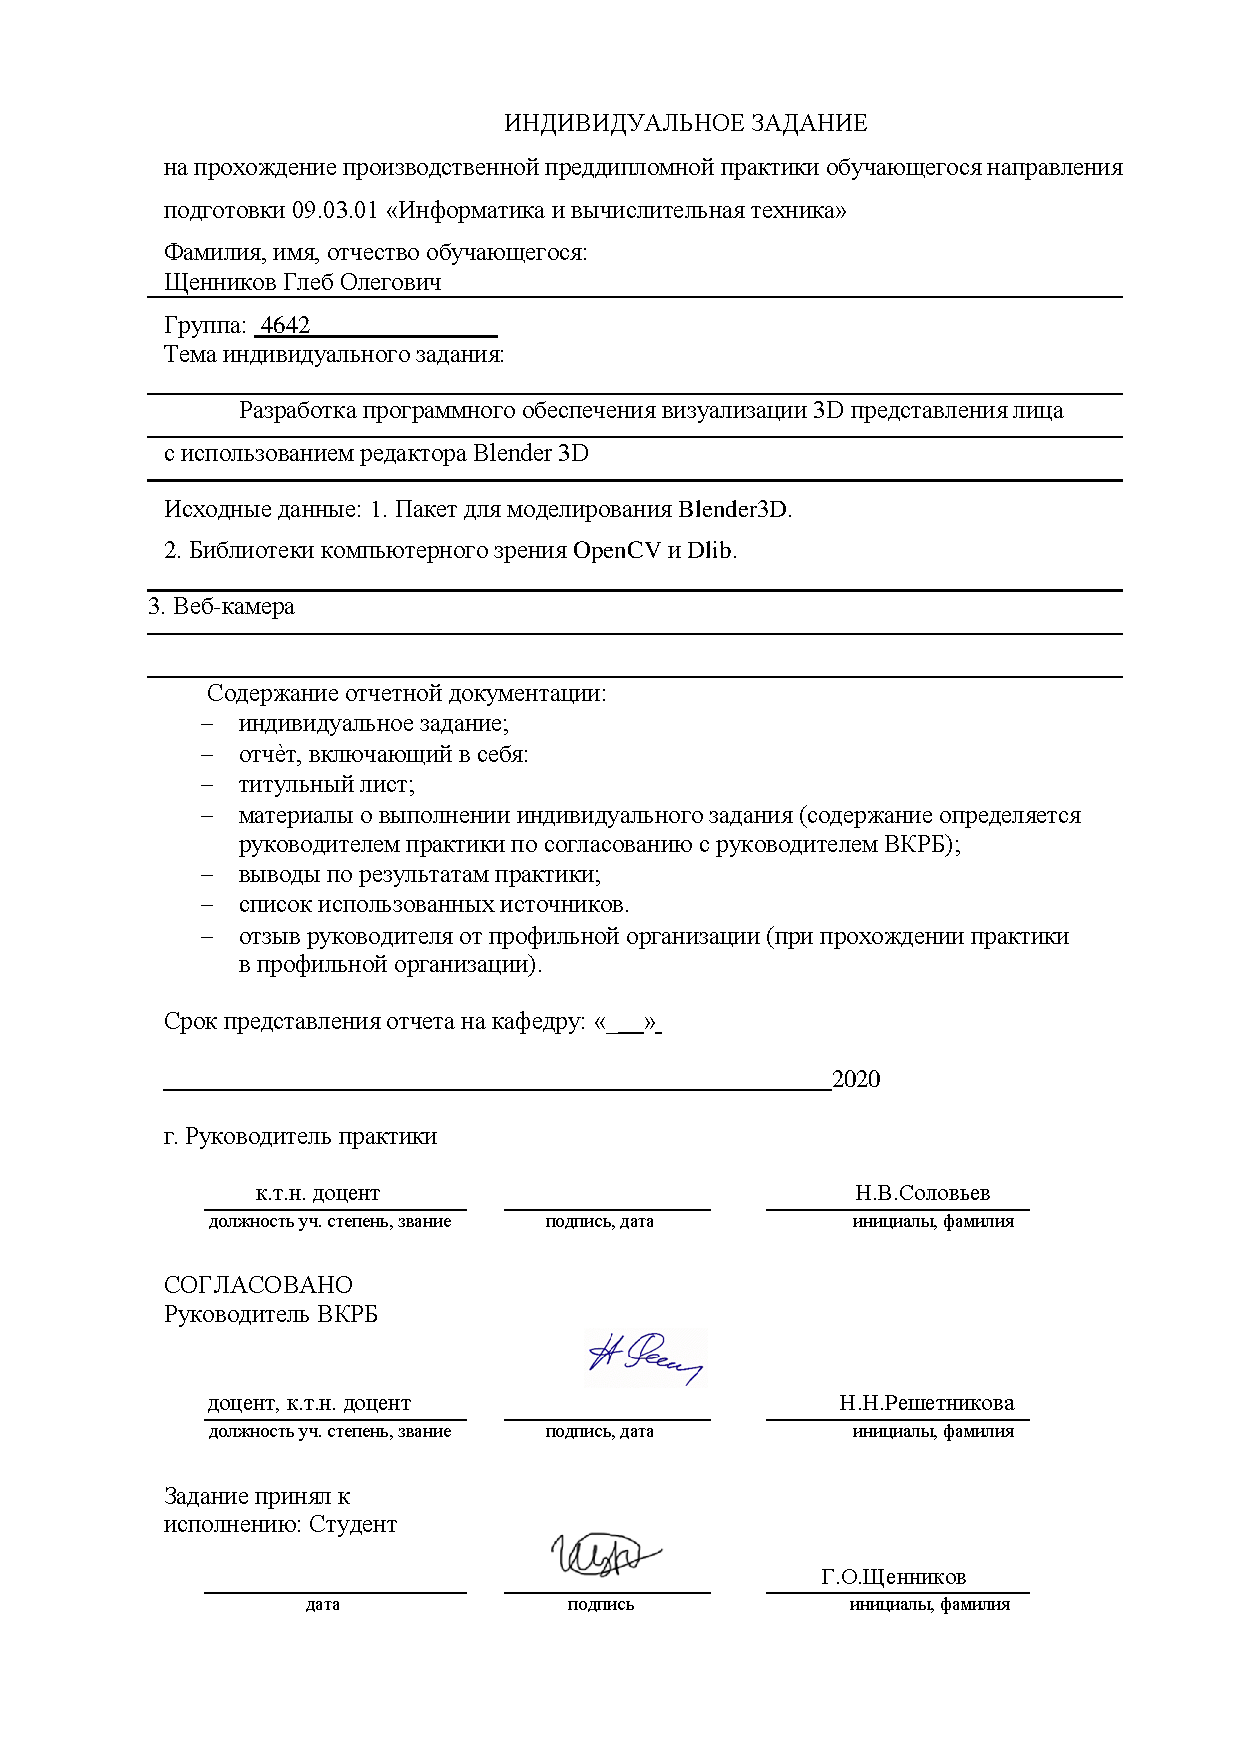
\includepdf{iz} % Индивидуальное задание
%
\includepdf[pages={1,2}]{task} % Задание на диплом печатается на одном листе с двух сторон
%помимо ПЗ и задания, в диплом также вкладывается отзыв руководителя и рецензия

%В рамках практики будет рассмотрен только этап обзора и выбора оступных средств пакета Blender.
%\tableofcontents % Содержание 
%\addtocontents{toc}{\protect\thispagestyle{empty}}
%\clearpage

\pagestyle{empty}
{
	\renewcommand{\thispagestyle}[1]{}
	\tableofcontents
}
\clearpage
\pagestyle{plain}

% Нумерация страниц по центру снизу
\pagestyle{fancy}
\fancyhf{}
\fancyfoot[C]{\thepage} % Page numbering for center header  
\fancyheadoffset{0mm}
\fancyfootoffset{0mm}
\setlength{\headheight}{17pt}
\renewcommand{\headrulewidth}{0pt}
\renewcommand{\footrulewidth}{0pt}
\fancypagestyle{plain}{ 
	\fancyhf{}
	\rhead{\thepage}
}

%\pagestyle{empty}
%\tableofcontents
%\clearpage
%\pagestyle{plain}

\anonsection{Перечень обозначений и сокращений}

ПО -- программное обеспечение

EAM -- Enterprise Asset Management - система управления активами

Фреймворк -- программная платформа, определяющая структуру программной системы; программное обеспечение, облегчающее разработку и объединение разных компонентов большого программного проекта.

Makespan -- период времени, который проходит от начала работы до ее завершения.

Job-shop -- оптимизационная проблема в информатике и исследовании операций. Это вариант оптимального планирования заданий. В общей проблеме планирования заданий нам дается $n$ заданий $J_{1}, J_{2}, ..., J_{n}$ с различным временем обработки, которые должны быть запланированы на $m$ машинах с различной вычислительной мощностью, при этом мы пытаемся минимизировать время выполнения (makespan) - общую длину расписания.

SQL -- structured query language - декларативный язык программирования, применяемый для создания, модификации и управления данными в реляционной базе данных, управляемой соответствующей системой управления базами данных.

.NET -- это бесплатная, кроссплатформенная платформа для разработчиков с открытым исходным кодом для создания различных типов приложений.

ORM -- Object-Relational Mapping - объектно-реляционное отображение, технология программирования, которая связывает базы данных с концепциями объектно-ориентированных языков программирования, создавая «виртуальную объектную базу данных».

ADO.NET -- ActiveX Data Object для .NET - технология, предоставляющая доступ к данным и управление ими, хранящимися в базе данных или других источниках.

Entity Framework -- ORM фреймворк с открытым исходным кодом для ADO.NET.

LINQ -- 
\clearpage
 % Перечень обозначений и сокращений
\anonsection{Введение}

\textbf{\textit{Актуальность.}}

ЕАМ-системы - чрезвычайно важная часть производственного процесса предприятий. Это инструмент управления производительностью, рисками и затратами, связанными с физическими (производственными) активами организаций.

Для современных производственных процессов актуальными являются задачи
оптимизации: оптимизация маршрутов логистики, рабочего времени, производственных
затрат и т. д. Масштаб таких оптимизационных задач может быть непосилен для решения
сугубо человеческими ресурсами, даже при использовании ЕАМ-систем, поэтому необходимо включать в область решения данных задач программно-аппаратные комплексы, решающие подобные задачи.

С 2011 года мировыми конгломератами ставится вопрос о четвертой промышленной революции - индустрии 4.0. Отходя от её утопических идей, индустрия 4.0 это гигантский шаг в сторону модернизации всех аспектов производства.

Большие данные, интернет вещей, блокчейн, искусственный интеллект, цифровые двойники - все эти технологии, которые уже нашли те или иные способы применения в различных областях науки и техники, только и ждут своего часа применительно к производству и производственным процессам. Уже сейчас самые передовые производства невероятно трудно представить без всех этих технологий.

Так новый передовой завод Intel (ссылка на видос Линуса) - полностью автоматизированное цифровое производство, где все самые важные и ответственные роли исполняют именно роботизированные механизмы или автономные дроны с интеллектом роя.

Умная фраза в заключение актуальности


\textbf{\textit{Степень разработанности темы, научно-техническая проблема.}}

На текущий момент на рынке представлено достаточно много решений, связанных с EAM и ERP системами,  как отечественные:

\begin{itemize}
	\item "TRIM"
	\item 1C ERP
	\item "Галактика ERP"
\end{itemize}

так и зарубежные:

\begin{itemize}
	\item SAP ERP
	\item IBM Maximo
\end{itemize}

Все представленные EAM-системы (как отдельные, так и в составе ERP) позволяют в полуавтоматическом режиме планировать работы, то есть указать какое количество ресурсов и когда понадобится для обслуживания тех или иных активов.

Во всех приведённых выше системах данное планирование происходит по потребности, то есть в долгосрочной перспективе не учитывает внезапные изменения, которые могут произойти с ресурсами, и их всевозможные коллизии - ситуации, когда в один момент времени один и тот же ресурс может быть задействован в разных работах.

Исходя из этого можно сказать, что в таких системах стоит до сих пор нерешенная проблема актуализации ресурсного планирования. Именно решение этой проблемы является целью данной работы.

\textbf{\textit{Объект работы}}

В качестве объекта работы выступают данные, полученные из системы класса EAM, структурированные определенным образом. В общем виде - база данных с набором сущностей вида "работа", "тип работы, "исполнитель" и так далее.

\textbf{\textit{Цель работы и решаемые задачи исходя из темы.}}

Цель данной работы - создание открытого мультиплатформенного решения, предназначенного для ресурсного планирования в системах управления физическими активами.

В данной работе решается задача ресурсного планирования, то есть распределение заданий по исполнителям в заданном временном интервале с учетом ограниченного количества имеющихся ресурсов.

\textbf{\textit{Планируемый н/т и практический уровень разработки, связь данной
	работы с другими.}}

В результате работы планируется получить готовое программно-техническое решение, которое может взаимодействовать с имеющимися EAM-системами и обеспечивать для них решение задачи ресурсного планирования с заданными граничными условиями.

\textbf{\textit{Методы или методология проведения работы.}}

\textcolor{red}{Убираем этот блок совсем.}

\textbf{\textit{Структура работы.}}

Работа состоит из Введения, N глав и Заключения, содержит список литературных источников из M наименований и Приложения/ий.

\clearpage
 % Введение
\section{Анализ предметной области разработки, сравнение с аналогами}

\subsection{Описание предметной области с анализом существующих решений и их недостатков исходя из целей работы и критериев сравнения, которые должны соответствовать искомым решениям поставленных задач.}
Одной из областей в операционных исследованиях является составление и оптимизация расписаний. Когда количество работ, человеческих ресурсов и различных механизмов невелико, то составление расписания вполне посильная для человека задача. Но когда количество объектов, учитываемых при планировании, возрастает, например, до уровня предприятия, то задача перестаёт быть тривиальной даже для целого отдела планирования. В таких случаях становится необходимым использование средств автоматизации планирования, примером которых являются мультиагентные системы или программные комплексы комбинаторной оптимизации - отдельные или в рамках ЕАМ-систем.

В целом можно разделить существующие методы построения и оптимизации подобных моделей на два основных подтипа - Мультиагентные системы (МАС) и Исследование операций (Operations research - далее OR) в рамках целочисленного программирования (программирования в ограничениях).

\subsubsection{МАС}

Мультиагентная система – система, состоящая из множества взаимодействующих друг с другом агентов. Каждый агент в такой системе независим и не имеет представления о системе в целом, но знает свои задачи и потребности, а также задачи и потребности агентов на одном с ним уровне. Для простоты понимания можно условно сказать, что агенты представляют собой нечто схожее с NPC (от англ. Non-Player Character - Неигровой персонаж) в компьютерных играх.
\comment{}{Перевод с английского}

Мультиагентные системы начали широко развиваться в девяностых годах и достигли своего пика к середине двухтысячных годов, после чего парадигма создания агентных сетей как чего-то, требующего отдельных подходов умерла в связи развитием и упрощением программирования в целом.

Согласно статьи Virginia Dignum и Frank Dignum \cite{vfdignum}, несмотря на существование целых организаций по изучению мультиагентных систем, ни за время существования этих организаций, ни за время их работы, МАС не смогли проявить себя ни в одной из заявленных областей, кроме как моделирования поведения персонажей в компьютерных играх \cite{masgames}. Исследователи связывают неудачу МАС со слабой способностью конкурировать с другими компьютерными технологиями того времени, в первую очередь вызванной тем, что из-под пера ассоциации или заинтересованных исследователей так и не вышло платформы МАС, которую могли бы использовать все желающие за пределами «закрытого» сообщества. Второй проблемой при попытке применить исследования агентов на практике, по их мнению, стала неспособность охватить или учесть существенные характеристики проблемы, для решения которой используются агенты. Аналогичные выводы были представлены Городецким и Скобелевым в статье 2017 года \cite{massuck}.
\comment{}{Убрал название статьи}

В целом всё-таки можно сказать, что МАС – достаточно перспективное направление, второе дыхание которому могут дать современные разработки в области искусственного интеллекта, нейросетей и программирования.

Главным плюсом (из которого в общих случаях следует и главный минус) мультиагентных систем является скорость реакции на изменения в системе и внешние факторы. Предполагается, что такая система фактически моментально должна реагировать на «происшествия» и сразу же выдавать удовлетворяющее решение с приемлемым качеством. Данное свойство мультиагентных систем делает их максимально пригодными для использования в качестве систем решения задач реального времени или в качестве модели-двойника.

Под моделью-двойником представляется виртуальный клон реальной системы, где все объекты взаимодействия являются агентами. Предполагается, что такие модели будут использоваться, например, для симулирования внештатных ситуаций в системе и оценки реагирования системы и агентов на эти ситуации. 

Так как МАС предлагают в целом «приемлемые решения», то в областях, где важна каждая мелочь и требуется наиболее полный точный результат, такой подход не подойдет. МАС вполне можно использовать на этапах конкретной эксплуатации, где как раз необходимы оперативные принятия решений, а вот в задаче установки оптимальных начальных условий такой подход скорее всего будет неприменим.

\subsubsection{Исследование операций}

Для получения наиболее точных и оптимальных решений применяется дисциплина под названием «Исследование операций». Согласно Википедии \cite{wikicp}, «ИО - дисциплина, занимающаяся разработкой и применением методов нахождения оптимальных решений на основе математического моделирования, статистического моделирования и различных эвристических подходов в различных областях человеческой деятельности. Иногда используется название «математические методы исследования операций».

Методы исследования операций являются основными в решениях таких задач как планирование, транспортные потоки, маршрутизация, упаковка и задачи о назначениях. В варианте, представленном в статье, предлагается использовать методы комбинаторной оптимизации, а именно – целочисленное программирование в ограничениях.

Программирование в ограничениях — это теория решения комбинаторных задач, опирающаяся на большое количество знаний из областей искусственного интеллекта, информатики и исследования операций. В программировании в ограничениях декларативно задаются ограничения для набора переменных входных данных. Ограничения не определяют последовательность действий для получения искомого результата, а указывают свойства и особенности для нахождения конечного результата. 

Оптимизация с ограничениями, или программирование с ограничениями (англ.- constraint programming, далее CP), — это название, данное идентификации выполнимых решений из очень большого набора возможных решений. CP основывается на выполнимости (нахождении выполнимого решения), а не на оптимизации (нахождении оптимального решения) и фокусируется на ограничениях и переменных, а не на целевой функции. Фактически, задача CP может даже не иметь целевой функции - цель может заключаться просто в том, чтобы сузить большое множество возможных решений до более управляемого подмножества путем добавления ограничений к задаче.

\subsection{Разработка возможных направлений проведения исследований и методов решений отдельных задач}
\comment{}{Подкорректирвал название}

Исходя из требований следует, что разработанная система будет предназначена для перепланирования некоторого множества предварительно заданных в ЕАМ-системе работ.

На текущий момент основным средством ресурсного планирования является фактически ручной метод распределения работ, при котором ответственные люди вручную указывают потребность в работах и ресурсах. При больших объемах работ при таком типе планирования теряется одна из важных потребностей планирования, а именно потребность в актуальности расписания.

Когда количество работ велико, становится физически невозможно одними человеческими силами отследить или как-то исправить пересечения в потребности тех или ресурсов, так как таких коллизий может быть сотни или тысячи даже на промежутке в неделю.

Решение данной проблемы программными средствами тоже сама по себе нетривиальная задача, так как в таком случае на систему необходимо смотреть в целом, а не разрешать отдельные коллизии, а каких-либо общепринятых адекватных решений для данной проблемы до сих пор представлено не было.

Исходя из вышесказанного одним из главных направлений проведения исследований в данной области будет анализ доступных средств и инструментов, подходящих под задачи ресурсного планировании, и вследствие исследование конкретных методов решения поставленных задач уже у выбранного направления.

\subsection{Обоснование применяемых технологий и инструментов.}
Реализация различных методов комбинаторной оптимизации представляется достаточно трудоемкой задачей, поэтому предполагается использование готовых библиотек и фреймворков, реализующих методы исследования операций.

Одними из самых популярных фреймворков для решения задач исследования операций являются открытые GLPK \cite{glpk}, LP\_Solve \cite{lpsolve}, MiniZinc \cite{minizinc}, Google OR-Tools \cite{ortools}, CHOCO \cite{choco} и проприетарные IBM CPLEX \cite{cplex} и Gurobi \cite{gurobi}.

К дальнейшему рассмотрению предлагается три из приведенных выше решений -- Открытый и бесплатный Google OR-Tools, как целевой фреймворк в данной работе, и проприетарные IBM CPLEX и Gurobi, как лидирующие решения в отрасли.
\comment{}{Обоснование выбранных для сравнения фреймворков}

Приведем частичные результаты бенчмарков между Google OR-Tools и IBM CPLEX, полученные в статье "Google vs IBM: A Constraint Solving Challenge on the Job-Shop Scheduling Problem" \cite{orvsplex}, в таблице 1.1.

\begin{table}[H]
	\caption{Сравнение Or-Tools и CPLEX в задаче Job-shop (меньше - лучше)}\label{orplextable}
	\begin{adjustbox}{width=1\textwidth}
		\begin{tabular}{|c|c|c|c|c|}
			\hline \multirow{2}{*}{Номер теста} & \multicolumn{2}{|c|}{Одно ядро} & \multicolumn{2}{|c|}{Четыре ядра} \\
			\cline{2-5} & CPLEX msp (sec) & OR-Tools msp (sec) & CPLEX msp (sec) & OR-Tools msp (sec) \\
			\hline 1 & 1234 (1.9) & 1234 (1.8) & 1234 (3.3) & 1234 (1.6) \\
			\hline 2 & 943 (0.7) & 943 (0.7) & 943 (1.4) & 943 (0.4) \\
			\hline 3 & 656 (1169.3) & 660 & 565 (525) & 661 (1200) \\
			\hline 4 & 682 & 679 & 680 & 679 \\
			\hline 5 & 685 & 695 & 694 & 689 \\
			\hline 6 & 55 (0) & 55 (0) & 55 (0) & 55 (0) \\
			\hline 7 & 930 (3.8) & 930 (5) & 930 (5.9) & 930 (2.9) \\
			\hline 8 & 1165  (1.4) & 1165 (5) & 1165 (0.5) & 1165 (3.4) \\
			\hline 9 & 666 (0) & 666 (0.1) & 666 (0) & 666 (0.1) \\
			\hline 10 & 655 (0.3) & 655 (0.3) & 655 (0.5) & 655 (0.1) \\
			\hline 
		\end{tabular}
	\end{adjustbox}
\end{table}

В тестах производительности между Google OR-Tools и IBM CPLEX стоял вопрос решения проблемы составления расписания работы в цехе (англ. Job-shop scheduling problem), которая приобрела особую известность благодаря своей простой формулировке, приводящей к трудно решаемым задачам.

Наиболее типичным критерием оптимизации является минимизация промежутка времени (англ. makespan), т.е. промежутка времени между началом первой операции и окончанием последней. Проблема представляется в виде набора заданий, которые должны быть обработаны набором машин. Каждое задание - это последовательность операций, каждая операция должна быть обработана определенной машиной и занимает определенное время обработки. Каждое задание имеет определенный порядок операций, который должен соблюдаться. Допустимым решением этой задачи является такая последовательность операций на каждой машине, при которой нет перекрытия времени между двумя операциями на одной машине и соблюдается порядок операций.

Как видим из статьи, по результатам тестов на момент 2017 года фреймворк IBM CPLEX в целом чаще выигрывал у OR-Tools в размере makespan и быстроте получения решения, при этом фреймворк OR-Tools показывал себя лучше в многоядерных тестах большого масштаба.

В другой статье \cite{mipshit} представлены уже результаты сравнения коммерческих IBM CPLEX и Gurobi. По результатам тестов последние версии обоих решателей в целом идут нога в ногу и выдают результаты очень близкие как по качеству, так и по скорости нахождения решений.

По результатам бенчмарков можно сказать, что между фреймворками Google OR-Tools, IBM CPLEX и Gurobi (особенно в многоядерной конфигурации) существует условный паритет по скорости и качеству решения оптимизационных задач, и в целом предугадать, кто окажется впереди в условиях реальной задачи невозможно.

Одним из наиболее доступных фреймворков является Google Or-Tools. OR-Tools - это программное обеспечение с открытым исходным кодом для комбинаторной оптимизации, которая направлена на поиск наилучшего решения проблемы из очень большого набора возможных решений. Последние несколько лет именно OR-Tools среди всех открытых библиотек занимает первые места в соревнованиях MiniZinc Challenge по программированию в ограничениях \cite{zincchal}. Также, в отличие от большинства остальных фреймворков имеет большее количество официально написанных интерфейсов под разные языки программирования – C++ (изначально написан именно на нём), C\#, Java, Python.

Фреймворк Google OR-Tools поддерживает решатели под задачи линейной оптимизации (решения проблемы, смоделированной как набор линейных зависимостей.), целочисленной оптимизации (Смешанное целочисленное программирование - Mixed Integer Programming – MIP; некоторые переменные обязательно представляют собой целые числа) и программирование в ограничениях. Все эти решатели могут быть использованы для решения таких задач, как: решение судоку, диета Стиглера \cite{stigler}, шахматные задачи, планирование, составление оптимальных маршрутов и т.д.

В результате обзора и анализа методов решения поставленной задачи, на данный момент наиболее подходящим методом можно признать метод комбинаторной оптимизации и программирования в ограничениях, так как он явно предоставляет набор устоявшихся практик и решений, показавших себя во множестве проектов.

Основным средством предлагается использовать фреймворк Google OR-Tools, решающий задачи комбинаторной оптимизации, так как данный фреймворк является бесплатным, открытым, может быть использован в коммерческой разработке и покрывает большую часть областей и задач исследования операций.

Мультиагентные системы на данный момент, напротив, по результатам анализа показали себя непригодными к повсеместному использованию, так как не предоставляют доступных средств для реализации и не были широко протестированы в реальных условиях.


\subsection{Уточненная постановка задачи и требования к прототипу решения.}
Имеются следующие начальные условия:
\begin{itemize}
	\item Есть множество запланированных работ (ЗР) на заданном временном интервале. Каждая работа имеет расчетные плановую дату/время начала выполнения и плановую дату/время завершения выполнения (разница между этими датами определяет длительность работы).
	\item Каждая работа имеет перечень исполнителей, необходимых для ее выполнения. Для каждого исполнителя задана потребность, выраженная в чел.*час.  В качестве исполнителя может быть указан один из конкретных исполнителей, имеющихся в штатном расписании.
	\item Имеется подразделение (цех, участок и т.п.), располагающее определенными людскими ресурсами. Состав людских ресурсов определяется штатным расписанием.
\end{itemize}
	Задача:
	
	На основании имеющихся исходных данных постараться построить такой порядок выполнения работ, чтобы в каждый день суммарная потребность в людских ресурсах и механизмах на выполнение всех работ не превышала объем располагаемых ресурсов, заданных в штатном расписании.
	
	Для того, чтобы найти такое решение, система может перемещать исходные ЗР во времени. При этом должны соблюдаться следующие условия:
	\begin{itemize}
		\item длительность работ и потребность в ресурсах, указанные для каждой ЗР, должны сохраняться;
		\item порядок выполнения работ одного типа и для одного и того же объекта должен сохраняться;
		\item может быть задана плановость определенных типов работ.
	\end{itemize}

	Результат:
	
	В результате система должна предложить новые плановые даты выполнения каждой ЗР при условии соблюдения заданных ограничений. Если решения нет, то система должна сообщить об этом, желательно при этом указать, какого ресурса или механизма (по мнению системы) недостаточно для выполнения плана.
	

\subsection{Выводы}

Были проанализированы два подхода к решению проблемы планирования в системах управления активами. Так как в самых популярных на сегодняшний день ЕАМ-системах, таких как 1С ERP, "ТРИМ", зарубежных SAP и Maximo есть лишь стандартные полуавтоматические способы планирования работ, то одним из самых востребованных направлений по улучшению такого функционала является полностью автоматическое планирование по заданным потребностям с учетом актуального распределения ресурсов.

Двумя самыми подходящими для такого функционала подходами являются мультиагентные системы и программирование в ограничениях. По результатам анализа подход с применением мультиагентных систем сложно рассматривать в качестве основного для данного типа задач, так как до сих пор, в том виде в каком он был представлен изначально, не показал реальных практических результатов, а также не было представлено каких-либо общедоступных сред для мультиагентного программирования. Программирование в ограничениях, напротив, предоставляет наиболее понятный набор инструментов и практик, поэтому для решения проблемы ресурсного планирования был выбран именно такой подход.


\clearpage

\section{Проектирование}

Проектирование планировщика ресурсов предполагает собой разработку, состоящую из следующих этапов:
\begin{itemize}
	\item анализ доступных средств платформы .Net;
	\item выбор типа базы данных и её провайдера;
	\item определение алгоритмов, по которым будет работать программный модуль;
	\item написание и отладка программного модуля.
\end{itemize}


\subsection{Проектирование архитектуры прототипа системы решения, включая разработку структуры (компоненты и связи между ними), внутреннего и внешнего функционирования.}

\subsubsection{Анализ доступных средств платформы .Net}

На данный момент платформу .Net можно условно поделить на две части - .Net Framework и .Net Core.

На данный момент платформа .Net Framework является поддерживаемой, но устаревшей, и по рекомендациям Microsoft \cite{microrec} не следует начинать новые проекты на этой платформе. Дополнительно необходимо указать, что платформа .Net Framework не является кроссплатформенной и работает только в операционных системах семейства Windows, что существенно ограничивает возможности современной разработки на ее основе на данный момент.

Открытый кроссплатформенный фреймворк .Net Core является преемником .Net Framework. Именно Core версию Microsoft рекомендует для всех новых проектов. Главным отличием новой платформы в первую очередь стала поддержка работы в Unix-системах (Linux, MacOS), соответственно все сервисы, написанные на .Net Core, без каких-либо ограничений могут быть использованы в современной серверной парадигме: Linux серверы, Docker, контейнеризация и виртуализация.

Для данного проекта была выбрана самая акутальная версия фреймворка .Net Core - .NET 6, так как она является LTS-версией, а так же соответствует всем требованиям проекта - открытости и кроссплатформенности.

В качестве платформы для взаимодействия с пользователем был выбран серверный вариант фреймворка Blazor. Blazor - это бесплатный и открытый фреймворк для написания веб приложений на языке C\#, поддерживающий реактивность, то есть работающий напрямую с DOM-элементами, а не HTML страницами. Blazor делится на Blazor WebAssembly - полностью клиентское приложение и на Blazor Server - клиент-серверную реализацию, в которой пользовательская и серверная часть общаются между собой по протоколу SignalR. SignalR - это бесплатная библиотека с открытым исходным кодом для Microsoft ASP.NET, которая позволяет серверному коду отправлять асинхронные уведомления веб-приложениям на стороне клиента. Библиотека включает в себя серверные и клиентские компоненты JavaScript.



\subsubsection{Определение алгоритмов, по которым будет работать программный модуль}

За планирование и/или перепланирование в планировщике будет отвечать библиотека Google OR-Tools. Задача, изложенная выше в первой главе, однозначно подходит под определение задач целочисленного программирования в ограничениях, так как каждый объект виртуальной модели в данной задаче можно определить как целочисленную переменную или их множество, на которые в явном виде можно наложить ряд ограничений и целевых функций, соответствующих условиям задачи.

Для такого типа задач пакет Google OR-Tools предоставляет отдельный класс для решения задач целочисленного программирования в ограничениях - CP-SAT, где CP (от англ. Constraint Programming - Программирование в ограничениях) - непосредственно целочисленное программирование в ограничениях, а SAT (от англ. Satisfiability - Удовлетворимость) - указывает, что целью решения данного класса задач является не нахождение одного конкретного результата, а нахождение одного или нескольких решений, удовлетворяющих ограничениям, наложенным на входные данные.
 
\subsubsection{Выбор типа базы данных и её провайдера.}

В первую очередь при выборе типа баз данных встаёт вопрос об использовании реляционных или нереляционных баз данных. В целом в EAM-системах обычно используются именно реляционные базы данных, так как этому способствует необходимость в четкой иерархической структуре модели представления активов предприятия. Также в EAM-системах редко встречается необходимость в шардинге - то есть в горизонтальном расширении данных для обеспечения масштабируемости. Исходя из этого для данного проекта была выбрана именно реляционная база данных.

В качестве реляционной СУБД был выбран PostgreSQL. PostgreSQL - это бесплатная система управления реляционными базами данных с открытым исходным кодом, в которой особое внимание уделяется расширяемости и соответствию стандарту SQL.

В данный момент ввиду острой необходимости в импортозамещении и независимости от зарубежных ПО, сервисов и средств именно СУБД PostgreSQL видится лучшим вариантом. У российских разработчиков уже есть большой опыт в развитии своих доработок и ответвлений PostgreSQL. Так, например, давно и успешно применяется ответвление Postgres Pro \cite{postgrespro}, СУБД ЛИНТЕР-ВС на базе PostgreSQL используется в ОС МСВС, а в дистрибутив операционной системы Astra Linux Special Edition (версия для автоматизированных систем в защищённом исполнении, обрабатывающих информацию со степенью секретности «совершенно секретно» включительно) включена СУБД PostgreSQL, доработанная по требованиям безопасности информации. Особенно важно, что СУБД Postgres PRO входит в реестр российского ПО \cite{reestrpp}.

\subsubsection{Проектирование архитектуры}

Желаемая архитектура системы представлена на рисунке \ref{arch}. Предполагается, что разрабатываемая система ресурсного планирования будет являться отдельным сервером планирования, работающим независимо от ЕАМ-системы. Связь между ЕАМ-системой и сервером планирования должна осуществляться посредством наличия общей базы данных и API для передачи команд и промежуточных объектов.

\addimghere{arch}{1}{Архитектура системы.}{arch}

Архитектуру самого сервера планирования (рис. \ref{archsp}) можно представить как API, который посредством контроллера вызывает сервис перепланирования, использующий библиотеку OR-Tools.

\addimghere{archsp}{0.7}{Архитектура сервера планирования.}{archsp}

Рассмотрим представленную на рисунке \ref{archsp} архитектуру сервера планирования более подробно.

Фронтенд (EAM-система) отправляет команду через API, в котором в привязанном к маршруту контроллере выполняются определенные действия - инициализация перепланирования выбранных через фронтенд работ или их же, но уже перепланированных, отправка обратно во фронтенд (ЕАМ-систему) на отображение и подтверждение.

Фактически самой главной частью представленного сервера планирования является сервис OR-Tools. Именно данный сервис отвечает за основную часть - непосредственно процесс планирования предварительно заданных работ. В данном сервисе происходит инициализация модели, задание ограничений для этой модели, а также задается целевая функция, то есть функция, относительно которой будут искаться все удовлетворяющие ограничениям решения для данной модели.


\subsection{Разработка прототипов алгоритмов, структур данных.}

\subsubsection{Типы данных Google OR-Tools}

Все объекты, для которых проводится процесс оптимизации, должны быть представлены в фреймворке Google OR-Tools одним из следующих типов данных:

\begin{itemize}
	\item IntVar; 
	\item BoolVar;
	\item IntervalVar;
	\item OptionalIntervalVar.
\end{itemize}

Тип данных IntVar это объект, который может принимать любое целочисленное значение в определенных диапазонах, такой диапазон называется доменом. В коде объявляется как
%\begin{lstlisting}
%	var integer_variable = model.NewIntVar(0, 100, "Integer Varible");
%\end{lstlisting}
\mint[breaklines]{csharp}|var integer_variable = model.NewIntVar(0, 100, "Integer Varible");|
где 0 и 100 это домен переменной, а "Integer Variable" - произвольное имя переменной, задаваемое пользователем.

Тип данных BoolVar представляет собой переменную для хранения логических значений. Внутри фреймворка BoolVar аналогичен типу IntVar, но с доменом $[0, 1]$. Выделен в отдельный тип данных для удобства программирования.

Пример объявления:
%\begin{lstlisting}
%	var boolean_variable1 = model.NewBoolVar("Boolean Variable");
%\end{lstlisting}
\mint[breaklines]{csharp}|var boolean_variable1 = model.NewBoolVar("Boolean Variable");|
В качестве параметров при объявлении передается только произвольное имя переменной, так как домен по умолчанию лежит в пределах $[0, 1]$

Тип IntervalVar представляет собой интервальную переменную. Интервальная переменная - это и ограничение, и переменная. Она определяется тремя целочисленными переменными: start, size и end.

Она является ограничением, потому что внутри она обеспечивает выполнение того, что start + size == end.

Это также переменная, поскольку она может задаваться в определенных методах ограничения планирования, таких как: NoOverlap, NoOverlap2D, Cumulative.

Объявляется так:
%\begin{lstlisting}
%	var interval_variable = model.NewIntervalVar(start, size, end, "Interval Variable");
%\end{lstlisting}
\mint[breaklines]{csharp}|var interval_variable = model.NewIntervalVar(start, size, end, "Interval Variable");|
в которой start - предполагаемый момент начала интервала, size - размер (длина) интервала - обычно фиксированное целое число, end - предполагаемый момент окончания интервала. 

В качестве значений start и end могут приниматься либо целые числа - в таком случае, например, суть оптимизации такой переменной заключается в нахождении её места на горизонте планирования, либо переменные типа IntVar - тогда оптимизация данной переменной будет зависеть и от также неизвестных переменных определенного домена.

Последним из доступных типов является OptionalIntervalVar - опциональный интервал. Этот отличается от IntervalVar литералом is\_present, который указывает, активна (то есть фактически присутствует в модели и участвует в процессе оптимизации) данная переменная или нет.

Пример:
%\begin{lstlisting}
%	var optional_interval_variable = model.NewOptionalIntervalVar(start, size, end, is_presernt "Optional Interval Variable");
%\end{lstlisting}

\mint[breaklines]{csharp}|var optional_interval_variable = model.NewOptionalIntervalVar(start, size, end, is_present "Optional Interval Variable");|
в которой is\_present представляет собой логическая переменную типа BoolVar.

Представленные выше типы данных определяются как часть модели. Модель это некоторое условное пространство имён, которое содержит в себе переменные-объекты модели, методы для работы с объектами, ограничения для них, а также методы для задания целевой функции модели.

Решение модели эквивалентно нахождению для каждой переменной единственного значения из множества начальных значений (называемого начальной областью), такого, что модель выполнима, или оптимальна, если вы предоставили целевую функцию.

Основными ограничениями для модели можно выделить:
\begin{itemize}
	\item Add; 
	\item AddNoOverlap;
	\item AddAllDifferent;
	\item AddImplication.
\end{itemize}

Метод Add добавляет ограничение в виде линейного выражения вида $x + y = z$, где $x, y, z$ - целые числа или переменные типа IntVar.

Ограничение AddNoOverlap гарантирует, что все выбранные для него интервалы не пересекаются во времени.

AddAllDifferent заставляет все переменные иметь разные значения.

Метод AddImplication обеспечивает ограничение вида ЕСЛИ, ТО - $a => b$.

Класс LinearExpr позволяет производить над типами данных OR-Tools различные математические операции, такие как сумма, скалярное произведение, умножение на коэффициент - Sum(), ScaleProd(), Term().

Для задания целевой функции фреймворк предлагает два метода - maximize и minimize. Данные методы позволяют максимизировать или минимизировать некоторые необходимые параметры модели.


\subsubsection{Определение требований к модели}

Так как при планировании работ периоды занятости ресурсов могут накладываться друг на друга независимо от качества планирования, то ожидается, что не все работы окажутся запланированными. Соответственно, цель работы планировщика заключается в максимизации количества запланированных работ и выражается формулой:

% Далее идёт расшифровка параметров, входящих в формулу
\begin{minipage}[h]{1\textwidth}
	\begin{equation}
		\max\sum_{0}^{N}(n_{0}, ..., n_{N})
	\end{equation}
	\begin{tabular}{llll}
		где & $N$ & {---} & количество работ; \\
		& $n$ & {---} & \begin{tabular}[t]{@{}l@{}}переменная домена $[0,1]$, означающая присутствие работы.\end{tabular}
	\end{tabular}
\end{minipage}

\bigbreak
Так как работы одного типа и работы, привязанные к одному человеку, никак не должны пересекаться, то должно так же выполняться следующее ограничение:

\begin{minipage}[h]{1\textwidth}
	\begin{equation}
		\forall p \in I \enspace \forall q \in I: p \neq q \implies V_p \cap V_q \neq \emptyset
	\end{equation}
	\begin{tabular}{llll}
		где & $V_i$ & {---} & семейство интервалов; \\
		& $p, q$ & {---} & \begin{tabular}[t]{@{}l@{}}интервал множества $V$.\end{tabular}
	\end{tabular}
\end{minipage}

\bigbreak
Из дополнительных ограничений следует отметить:

Для каждого рабочего количество запланированных работ должно быть меньше или равно изначальному количеству.

Так как в типах работ присутствуют плановые работы, то для работ таких типов должна соблюдаться определенная периодичность, например, планирование раз в день, неделю, месяц и так далее.

\clearpage

%\section{Реализация предлагаемого решения и его оценка}

Реализация системы ресурсного планирования состоит в описании модели методами целочисленного программирования, интеграции этой модели в сервис планирования и написания подобия EAM-фронтенда, который будет взаимодействовать с сервисом, то есть отображать исходные данные, запускать процесс перепланирования, отображать результаты работы сервиса, а также различную статистику.

\subsection{Реализация прототипа технического решения}

\subsubsection{Описание инструментов и форматов данных}

В качестве среды программирования была выбрана Visual Studio 2022 под операционной системой Windows 11.

Библиотека Google Or-Tools поставляется из официального NuGet репозитория.

Как сервис ресурсного планирования, так и частичный функционал подобия ЕАМ-системы будут реализованы с помощью Blazor Server.

Данные о ресурсах и работах будут храниться в реляционной базе данных PostgreSQL, взаимодействие с базой данных извне будет происходить через SQL клиент DBeaver, а внутри проекта через ORM Entity Framework Core.

Структурная схема использованных инструментов представлена на рисунке \ref{instruments}.

\addimghere{instruments}{0.8}{Структура взаимосвязей инструментов.}{instruments}

\subsubsection{Описание модели базы данных}

Схема реляционной базы данных, достаточной для описания модели, представленной в главе 1 представлена на рисунке \ref{schema}.

\addimghere{schema}{1}{Схема базы данных.}{schema}

В схеме представлены следующие сущности:
\begin{itemize}
	\item jobs
	\item jobtypes
	\item workers
	\item jobsworkers
\end{itemize}

Сущность jobs представляет все работы, запланированные на текущий момент времени.

Сущность jobtypes представляет все доступные типы работ. Связана с сущностью jobs связью один ко многим.

В таблице workers находятся все рабочие, которые могут быть привязаны к работам. Связана с таблицей jobs связью многие ко многим, поэтому необходимо использование промежуточной таблицы jobsworkers.

\subsubsection{Прототипирование ЕАМ-системы}

Для упрощения взаимодействия с сервисом планирования, а так же для упрощения написания вспомогательных инструментов, в качестве платформы для ЕАМ-системы был выбран веб-фреймворк Blazor Server.

При использовании модели хостинга Blazor Server приложение выполняется на сервере из приложения ASP.NET Core. Обновления пользовательского интерфейса, обработка событий и вызовы JavaScript обрабатываются через соединение SignalR.

Данный фреймворк позволяет создавать реактивные веб-приложения без использования языка JavaScript и его фреймворков, что значительно упрощает и ускоряет разработку веб-приложений для .Net программистов, не владеющих стеком технологий, таких как JavaScript, Angular, React и подобных.

Желаемый вид ЕАМ-системы представлен на рисунке \ref{interface}:

\addimghere{interface}{1}{Желаемый интерфейс прототипа ЕАМ-системы}{interface}

На рисунке показано основное окно системы - окно планирования работ, в котором находятся элементы управления для выбора плановых дат, перепланирования и записи результата в базу данных. Основным информационным элементом на данной странице является диаграмма Ганта.

Страница "Домой" служит для отображения основной информации о прототипе системы, страницы "Типы работ" и "Персонал" служат только для отображения исходных данных по сущностям "Типы работ" и "Персонал".

Диаграмма Ганта - столбчатая диаграмма, которая используется для иллюстрации плана или графика работ, например, во времени. Данный тип диаграмм повсеместно используется в системах подобного класса и очень удобен для отображения информации данного типа.

Так как диаграмма Ганта достаточно сложный к реализации элемент, было принято решение использовать его готовую реализацию. Готовая реализация была взята из пакета Syncfusion \cite{syncblazor}, который бесплатно предоставляет ряд веб-компонент для некоммерческого использования и для студентов. Вид диаграммы из пакета Syncfusion Blazor представлен на рисунке \ref{syncgantt}.

\addimghere{syncgantt}{1}{Компонент диаграммы Ганта из пакета Syncfusion}{syncgantt}

Пакет готовых форм Syncfusion предоставляет возможность отображения работ одного типа в одной строке только в версии для фреймворка Angular, поэтому в данном прототипе каждая работа представлена отдельной строчкой на диаграмме.

Итоговый вид основного окна представлен на рисунке \ref{eammain}.

\addimghere{eammain}{1}{Страница планирования работ прототипа ЕАМ-системы}{eammain}

От кнопки сохранения перепланированных работ было решено отказаться, так как данный функционал не является необходимым для выполнения данной работы.

Остальные страницы прототипа представлены на рисунках \ref{homepage}, \ref{jobtypes} и \ref{staff}.

\addimghere{homepage}{1}{Домашняя страница прототипа}{homepage}

\addimghere{jobtypes}{1}{Страница "Типы работ"}{jobtypes}

\addimghere{staff}{1}{Страница "Персонал"}{staff}

Главным преимуществом использования фреймворка Blazor в подобных проектах является отсутствие необходимости в знании каких-либо дополнительных языков и их средств, например, JavaScript и React - вся реализация веб-приложения состоит целиком из HTML/CSS и кода на языке C\#.

В качестве примера можем рассмотреть страницу планирования работ. Данная страница состоит из двух частей: Razor страницы/компонента с расширением .razor или .cshtml и вспомогательного кода, наподобие модели-представления из паттерна MVVM. Вспомогательный код может находится либо прямо внутри представления, либо отдельным файлом как составной класс данного представления. Такая структура представлена на рисунке \ref{blazstruct}.

\addimghere{blazstruct}{1}{Структура razor-страниц}{blazstruct}

Как видно из рисунка выше, в представлении Gantt.razor задан HTML-код со вставками на C\#. Данные вставки берутся из методов и свойств составного класса Gantt.razor.cs и позволяют реактивно менять значения на странице.

\subsubsection{Моделирование системы средствами программирования в ограничениях}

Все действия по планированию и/или перепланированию работ происходят на горизонте планирования, который выбирается пользователем и в рамках данной работы определятся целочисленным типом данных. Горизонт планирования рассчитывается в минутах и находится в диапазоне от 0 до 2,147,483,647 (ограничивается целочисленным типом данных языка C\#). Такой диапазон покрывает 4085 лет и является более, чем достаточным для всех реальных задач планирования в EAM-системах. Был выбран горизонт планирования в минутах, так как он обеспечивает достаточную точность относительно часов, а в численном виде значительно меньше секунд, что сократит необходимую память для планирования.

Для описания работ были выбраны следующие типы данных, доступные из библиотеки OR-Tools:
\begin{itemize}
	\item BoolVar
	\item IntVar
	\item OptionalIntervalVar
\end{itemize}

Тип данных IntVar в данной модели определяет переменные моментов начала и конца работ. Лежит в диапазоне от 0 до значения горизонта планирования.

Типом BoolVar определяется актуальность работы, то есть ее участие в процессе планирования. Данная переменная используется в типе OptionalIntervalVar. Переменная задается в диапазоне от 0 до 1 по умолчанию, соответственно если значение переменной равно единице, то работа учитывается при планировании, 0 - не учитывается.

OptionalIntervalVar уже определяет саму работу на горизонте планирования. В отличие от просто IntervalVar данный тип - опциональный и зависит от переменных типа BoolVar, используемых литералом is\_present.

Для составления модели до момента задания ограничений необходимо в первую очередь инициализировать работы, то есть инициализировать все переменные, представляющие работы.

В первоначальной версии модели инициализация была проделана так:
\begin{minted}{python}
for h in range(horizon)
    ...
    for w in workers
        ...
        for jt in job_types
            ...
            for job in jobs
\end{minted}

В данном варианте инициализация происходит относительно четырех сущностей модели: каждой минуты горизонта планирования, каждого рабочего, каждого типа работы и непосредственно каждой работы.

Отсюда, например, при 10 рабочих, 10 типах работ, 10 запланированных работах и горизонте планирования в 10080 минут (семь дней):

$10 * 10 * 10 * 10080 = 10080000$

Получаем некий объект, в котором уже для простейшего примера ресурсного планирования получим непомерно огромные затраты по памяти, причем полученную цифру в 10080000 необходимо еще умножить на 4, так как имеем при инициализации для каждой работы две переменных типа IntVar, одну BoolVar и одну OptionalIntervalVar, в итоге - свыше сорока миллионов объектов для простого тестового примера.

Необходимость в наличии инициализации относительно горизонта планирования была связана с недопониманием концепции использования опциональных интервалов. Изначально казалось необходимым наличие возможности начала работы в каждую из минут горизонта планирования, что соответственно добавляло лишнее измерение в инициализацию.

Тем не менее, такой подход оказался рабочим и выдавал удовлетворяющий результат, то есть соответствовал ограничениям и целевым функциям модели, откуда можем сделать вывод о возможности наличия более чем одного подхода в моделировании при решении проблем программирования в ограничениях.

Результаты исследований прототипа модели первой версии будут представлены ниже в соответствующей главе.

Во второй итерации модели, уже при переносе с языка Python на C\#, были найдены некоторые недочеты первой версии модели, а также пересмотрена процедура инициализации, в результате которой был убран цикл по горизонту планирования. Это обуславливается тем, что в интервальных переменных и так задается их момент возможного начала и момент возможного конца, соответственно нет необходимости в привязке начала интервалов к конкретному моменту горизонта планирования.

Итоговый вид инициализации на языке C\#:

\begin{minted}{csharp}
...
foreach (var w in workers)
{
    ...
    foreach (var jt in job_types)
    {
    ...
        foreach (var job in jobs)
        {
            if (jt == job.Type && w == job.WorkerID)
            {
                var performed_at = model.NewBoolVar($"performed by {w}wID {jt}type {job.ID}jID");
                var start = model.NewIntVar(0, horizon, $"start of {w} {jt} {job.ID}");
                var end = model.NewIntVar(0, horizon, $"end of {w} {jt} {job.ID}");
                var optint = model.NewOptionalIntervalVar(start, job.TimeSpanMinutes, end, performed_at, $"interval of {w} {jt} {job.ID}");
                ...
            }
        }
\end{minted}

Следующим шагом после инициализации входных данных для модели является задание ограничений.

Первая группа ограничений - работы одного типа, а так же работы одного рабочего не должны пересекаться.

Для этого языком подзапросов LINQ из переменных, представляющих входные данные необходимо достать необходимые работы. Для рабочих:
\begin{minted}{csharp}
//работы по рабочему
List<List<IntervalVar>> jobIntervals_by_worker = new();
foreach (var w in intervals_by_worker)
{
    var flatlist = w.SelectMany(i => i).ToList();
    jobIntervals_by_worker.Add(flatlist);
}

//работы одного рабочего не пересекаются
foreach (var ji in jobIntervals_by_worker)
{
    ji.AddRange(sleepIntervals);
    model.AddNoOverlap(ji);
}
\end{minted}

В данном примере следует обратить внимание на метод AddNoOverlap, который и устанавливает ограничение на непересечение элементов выборки ji, то есть множества работ одного рабочего.

Задание ограничений этой группы для работ одного типа происходит аналогично.

Дополнительно следует отметить, что для множества рабочих было задано дополнительное ограничение в виде работы только по будням с девяти утра до девяти вечера.

\begin{minted}{csharp}
    //определим нерабочие (ночные интервалы) - допустим с 9 утра до 9 вечера
    //даты планирования выбираются пользователем с 00:00 по 00:00
    //0 + 540 => ночь; +720 => день; + 180 => остатки ночи
    List<IntervalVar> sleepIntervals = new();
    int dayCounter = 0;
    
    foreach (DateTime day in EachDay(reftime, lastday))
    {   
        int st = dayCounter * 1440;
        if ((day.DayOfWeek == DayOfWeek.Saturday) || (day.DayOfWeek == DayOfWeek.Sunday))
        {
            //по выходным не работаем
            int fin1 = st + 1440;
            var siSS = model.NewIntervalVar(st, 1440, fin1, $"sat/sun {dayCounter}");
            sleepIntervals.Add(siSS);
        }
        else
        {
            //по будням - с 9 до 9
            int fin = st + 540;
            var si = model.NewIntervalVar(st, 540, fin, $"sleep 1 of day {dayCounter}");
            sleepIntervals.Add(si);
            st = fin + 720; //пропускаем рабочие 12 часов
            fin = st + 180;
            //второй ночной интервал
            var si2 = model.NewIntervalVar(st, 180, fin, $"sleep 2 of day {dayCounter}");
            sleepIntervals.Add(si2);
        }    
        dayCounter++;
    }
\end{minted}

Следующим шагом необходимо ограничить возможное количество работ. В данном варианте мы считаем, что перепланированное количество работ одного типа и количество работ у одного рабочего должно быть меньше или равно исходному их количеству. Тогда для работ одного типа:

\begin{minted}{csharp}
    ///разделяем performed_at по типам работы
    Console.WriteLine("разделяем performed_at по типам работы");
    List<List<IntVar>> performedAt_by_type = new();
    foreach (var t in job_types)
    {
        List<IntVar> perflist = new();
        performedAt_by_type.Add(perflist);
    }
    foreach (var b_worker in bools_by_worker)
    {
        for (int b_type = 0; b_type < b_worker.Count; b_type++)
        {
            var flatperf = b_worker[b_type];
            performedAt_by_type[b_type].AddRange(flatperf);
        }
    }
    for (int i = 0; i < performedAt_by_type.Count; i++)
    {
        model.Add(LinearExpr.Sum(performedAt_by_type[i]) <= job_type_num[i]);
    }
\end{minted}

Необходимое ограничение задается в строке \mintinline{csharp}|model.Add(LinearExpr.Sum(performedAt_by_type[i]) <= job_type_num[i])|, где метод Add() задает для модели некое линейное ограничение. Метод LinearExpr.Sum(), переданный в Add() позволяет производить над множествами объектов типа OR-Tools операцию сложения значений элементов множества. Соответственно данной строкой мы задаем для модели, что количество работ перепланированных меньше или равно количеству работ исходных.

Ограничение по количеству работ для конкретных рабочих задается аналогично.

Так как у работ может быть задана некая периодичность выполнения, например, каждый день, раз в неделю, раз в месяц и так далее, то необходимо задать механизм эту периодичность устанавливающий.

Изначально данное ограничение представлялось очень простым. У каждой работы (опционального интервала) заданы переменные start и end типа IntVar, обозначающие возможный момент начала и возможный момент окончания работы. Соотвественно ограничение выглядело тривиально: $start_{n+1} - end_n > X$, где $X$ - интервал, через который плановые работы одного типа должны выполняться.

Так как переменные start и end используются в опциональном интервале, то ожидалось, что при невозможности для двух работ соответствовать ограничению $start_{n+1} - end_n > X$ - данные работы просто не будут учитываться, так как привязаны к типу OptionalIntervalVar. В действительности же заданные ограничения при невозможности их удовлетворить делали всю модель невыполнимой, в связи с тем, что ограничения к данным переменным рассматриваются сами по себе и без привязки к другим типам в модели. Именно для таких случаев используются связывающие ограничения.

Связывающие ограничения (от англ. - channeling constraint) связывают переменные внутри модели. Они используются, когда необходимо выразить сложную связь между переменными, например, "если эта переменная удовлетворяет условию, то она заставляет другую переменную принять определенное значение".

В данном случае необходимо указать, что если ограничение $start_{n+1} - end_n > X$ выполнимо, то литерал is\_present, отвечающий за актуальность опционального интервала, станет равным единице, то есть работа с этим литералом будет учитываться при планировании.

Выражается таким образом:

\begin{minted}{csharp}
//для третьего типа (плановая работа) - работы не чаще раза в день
    ...
    if(type == 3)
    {
        for (int i = 0; i < startAt_by_type[k].Count - 1; i++)
        {
            for (int j = i+1; j < startAt_by_type[k].Count; j++)
            {
                //if (b-a>1440) => b=0
                model.Add(startAt_by_type[k][j] - endAt_by_type[k][i] >= 1440).OnlyEnforceIf(performedAt_by_type[k][i]);
            }
        }
        break;
    }
    ...    
\end{minted}

В этом примере с помощью метода OnlyEnforceIf() устанавливается, что если выполнятся ограничение в методе Add(), то переменная типа BoolVar внутри метода OnlyEnforceIf() обратится в 1.

Последним шагом остается задать целевую функцию. В качестве целевой функции предлагается максимизировать количество перепланированных работ в целом. Для этого напишем такой код:

\begin{minted}{csharp}
//возьмем множество всех работ
var flatbools = bools_by_worker.SelectMany(i => i).SelectMany(i => i);
//целевая функция - максимизировать количество работ
model.Maximize(LinearExpr.Sum(flatbools));
\end{minted}

В данном примере целевая функция задается через метод модели Maximize(), в который передается множество всех работ. В данном случае каждый объект элемент множества является типом данных BoolVar.


\subsection{Экспериментальные исследования прототипа решения}

После создания прототипа была проведена экспериментальная оценка пригодности системы для задач ресурсного планирования в соответствии с поставленной задачей.

Основные характеристики аппаратно-программной конфигурации, которая использовалась для создания прототипа: компьютер – AMD Ryzen 9 5900HX, видеокарта Nvidia GeForce RTX 3070 Laptop 8Гб, оперативная память 16Гб DDR4.

Основными критериями для исследований предлагается использовать:
\begin{itemize}
    \item Зависимость времени планирования от количества работ/ресурсов
    \item Зависимость требуемой памяти от количества работ/ресурсов
    \item Результативность алгоритма (процент количества перепланированных работ от исходного)
\end{itemize}

\subsubsection{Сравнение двух версий модели}

Для начала рассмотрим время планирования (рисунок \ref{1vs2time}) и требуемый объем памяти (рисунок \ref{1vs2ram}) для планирования 13 работ на горизонте в одну неделю для моделей первой и второй версии:

\addimghere{1vs2time}{0.8}{Разница во времени планирования для моделей первой и второй версии (меньше - лучше)}{1vs2time}

\addimghere{1vs2ram}{0.8}{Разница в требуемой оперативной памяти для моделей первой и второй версии (меньше - лучше)}{1vs2ram}

По графикам, представленным на рисунках \ref{1vs2time} и \ref{1vs2ram}, видно, что модель второй версии отрабатывает на порядок быстрее и требует на порядок меньше памяти. Время перепланирования первой модели составило 14 минут, второй модели - 5 секунд, для работы первой модели потребовалось 12 гигабайт оперативной памяти, а для работы второй - всего лишь 300 мегабайт.

Такая явная разница в результатах работы обусловлена, как было указано выше в части 3.1.4, наличием лишнего измерения при инициализации данных вследствие применения ошибочного подхода при моделировании.

Представленные выше графики показывают, что хотя результаты работы разных вариантов модели для одной и той же задачи могут быть удовлетворительными, далеко не все из них могут быть применимы в реальных условиях, так как по тем или иным причинам могут не соответствовать требованиям по памяти или быстродействию.

\subsubsection{Анализ работы итоговой версии модели}

Рассмотрим результаты работы второй (итоговой) версии модели.

В первую очередь проверим перепланирование в граничных условиях, для которых заранее известен результат планирования в соответствии с постановкой задачи.

Так как при моделировании были использованы нестрогие ограничения, мы точно можем сказать, что количество запланированных работ будет больше нуля при любых начальных условиях. Единственным вариантом, в котором представляется отсутствие перепланированных работ является вариант, где выбранный горизонт планирования меньше времени наименьшей работы. Такой вариант является нереалистичным и рассматриваться не будет.

Для тестирования работы в граничных условиях приведём вариант планирования работ нескольких типов на горизонте одного дня, где все работы назначены одному человеку и не могут выполниться в полном объёме не пересекаясь (рис. \ref{borderinit}).

\addimghere{borderinit}{0.9}{Заведомо неисполнимый вариант планирования потребности в работах}{borderinit}

По рисунку выше видно, что есть пять работ типов "Обход", "Ремонт", "Плановый осмотр", "Замена", которые явно следуют друг за другом и не пересекаются. Работы типа "Остановка" находятся в границах других работ и выполнены быть не могут.

Очевидно, что исходя из данной диаграммы Ганта как минимум пять работ должны остаться после перепланирования. Есть вероятность, что при данных начальных условиях работы можно перепланировать так, что их возможное непересекающееся множество будет состоять более чем из пяти интервалов, но уже даже на такой небольшой выборке видно, что для человека задача становится достаточно нетривиальной и потребует относительно долгое время на разрешение.

Результат перепланирвоания представлен на рисунке \ref{borderafter}. 

\addimghere{borderafter}{0.9}{Результат работы планировщика в граничных условиях}{borderafter}

Как видно из рисунка \ref{borderafter}, планировщик исключил самую длинную работу по замене, оставив вместо нее две работы по остановке, длинна которых эквивалентна работе по замене, тем самым увеличив количество запланированных работ. Непосредственно процедура перепланирования заняла меньше 1 секунды и потребовала 250 мегабайт оперативной памяти.

В интерфейсе прототипа ЕАМ-системы результат перепланирования (рис. \ref{bordeream}) выглядит так:
    
\addimghere{bordeream}{0.8}{Результат работы планировщика в граничных условиях в интерфейсе ЕАМ-системы}{bordeream}

В качестве второго граничного условия определим 100 случайно заданных работ на горизонте планирования в одни сутки.

По результатам тестирования в данных условиях перепланировать удалось лишь 51 из 100 работ. Визуальный осмотр результатов, сравнение диаграмм Ганта до и после, просмотр логов планировщика не выявили аномальных или подозрительных результатов, а перепланированные интервалы соответствовали поставленной задаче, поэтому можно сделать вывод, что в данном граничном эксперименте модель также отработала корректно.

При таких входных данных наиболее интересным для исследования оказался параметр времени перепланирования при разном количестве задействованных на алгоритм ядер процессора.

На рисунке \ref{procusage} показана зависимость времени планирования от количества используемых процессоров.

\addimghere{procusage}{0.9}{Зависимость времени планирования от количества задействованных ядер процессора}{procusage}

По результатам эксперимента выше видим, что количество задействованных процессоров является одним из самых важных факторов быстродействия в данной модели. При использовании множества процессоров, каждый из них выполняет свою часть по поиску решений из множества всех решений.

Анализируя результат эксперимента в граничных условиях можно сказать, что планировщик корректно отработал в рамках поставленной задачи, показав высокую скорость работы и относительно небольшие требования к оперативной памяти. При этом, ключевую роль в быстродействии алгоритма перепланирования сыграло количество задействованных процессоров, показавшее явный, фактически линейный тренд на уменьшение времени планирования при увеличении количества процессоров.

Рассмотрим зависимость метрик перепланирования от количества работ и горизонта планирования. Количество типов работ и рабочих для всех тестов будет оставаться неизменным и равным десяти. Типы работ, продолжительность и дата выбираются случайным образом.

На рисунках \ref{100jtime} и \ref{1000jtime} показано время в секундах, требуемое для перепланирования 100 и 1000 работ на горизонте от 31 до 365 дней.

\addimghere{100jtime}{0.9}{Зависимость времени планирования от количества задействованных ядер процессора}{100jtime}

\addimghere{1000jtime}{0.9}{Зависимость времени планирования от количества задействованных ядер процессора}{1000jtime}

По представленным графикам видно, что на требуемое время планирование всех работ сильно влияет выбранный горизонт планирования. Данная зависимость связана с тем, что на длительных интервалах горизонта планирования существует достаточно свободного места для всех работ, и планирование в таком случае становится достаточно тривиальным.

Соответственно, чем меньше задается выбранный интервал, тем меньше становится вариантов расположить необходимое количество работ, то есть сужается множество удовлетворяющих решений на всем возможном множестве решений.

По графику \ref{1000jtime} сильно заметно влияние использования нескольких процессорных ядер для процесса планирования. Перепланирование с 8 ядрами оказалось примерно в 8 раз быстрее одноядерного перепланирования, что также соотносится с результатами, полученными в тестировании граничных условий (рис. \ref{procusage}).

Проведем замеры скорости планирования в зависимости от количества работ на горизонте в один год. Так как работы выбираются и распределяются в случайном порядке, проведем эксперимент 10 раз и построим зависимость от среднего времени перепланирования.

График зависимости времени планирования от количества работ представлен на рисунке \ref{365d2k}:

\addimghere{365d2k}{0.9}{Зависимость времени планирования от количества работ}{365d2k}

Как видно из рисунка \ref{365d2k}, примерное количество работ, которое в кратчайшие сроки может быть запланировано на один год находится в промежутке от 0 до 1900 работ. В процессе тестирования был выявлен промежуток, в котором перепланирование начинало занимать больше часа времени - данный промежуток составил от 1900 до 2100 работ. Среднее время перепланирования в интервале до 1900 работ составило менее 10 секунд. Увеличение горизонта планирования до двух лет позволило завершить операцию перепланирования за 3 секунды.

Было проведено исследование зависимости времени перепланирования от количества доступных рабочих. При уменьшении их количества в два раза, количество работ, которые возможно перепланировать в короткие сроки так же уменьшилось в два раза, и находится в промежутке от 800 до 1100 работ. Увеличение же числа рабочих в два раза не повлияло на время перепланирования, исходя из чего можем сделать вывод о наличии некой границы, ограничивающей быстроту перепланирования для данной модели.

Одной из интересных метрик оказалась средняя плотность запланированных работ в день (рис. \ref{plotn10}), при которой модель справляется с перепланированием пределах двух-трех часов:

\addimghere{plotn10}{0.9}{График зависимости средней плотности планирования работ от горизонта планирования}{plotn10}

По графику, представленному на рисунке \ref{plotn10} видно, что для 10 типов работ средняя максимальная плотность перепланирования составила около 5.5 работ в день при горизонте планирования от 180 дней и более. Под максимальной плотностью в данном случае понимается такая плотность, которая достигается при количестве работ, перепланируемых не более чем за три часа. Высокая плотность в пределах 180 дней связана с тем, что за аналогичное время модель способна разместить большее количество работ при меньшем горизонте планирования.

Проверим зависимость времени перепланирования при 20 типах работ (рис. \ref{20jtsmall} и рис. \ref{20jtbig}):

\addimghere{20jtsmall}{0.9}{Зависимость времени планирования от количества работ при 20 типах работ}{20jtsmall}

\addimghere{20jtbig}{0.9}{Зависимость времени планирования от количества работ при 20 типах работ до момента подскока времени планирования}{20jtbig}

Проверим, сохранится ли вид графика плотности планирования при большем количестве типов работ. Исходя из результатов, полученных в экспериментах выше, график должен сохранить свою форму, а средняя плотность должна быть примерно в два раза больше.

График плотности от 20 типов работ представлен на рисунке \ref{plotn20}:

\addimghere{plotn20}{0.9}{График зависимости средней плотности планирования работ от горизонта планирования}{plotn20}

Как видно из рисунка \ref{plotn20}, форма графика соответствует форме графика плотности от 10 типов работ, а средняя плотность при долгосрочном планировании увеличилась в 2.4 раза, что так же соответствует ожиданиям.

Последней метрикой для рассмотрения выберем зависимость количества перепланированных работ от количества доступных рабочих. Аналогичный эксперимент с типами работ показал явную зависимость от изменения количества типов, поведение модель в данном эксперименте ожидается похожим.

На рисунке \ref{work20} представлены графики зависимости количества работ от горизонта планирования при разном количестве доступных рабочих:

\addimghere{work20}{0.9}{График зависимости средней плотности планирования работ от горизонта планирования}{work20}

Подобно закону Густафсона-Амдала, в данном случае больший интерес вызывает не быстродействие при определенном объеме вычислений, а объем вычислений при сходном времени. Как видим из рисунка \ref{work20}, в отличие от изменения количества типов работ, изменение количества доступных рабочих не так сильно повлияло на объем модели при сходном времени. Такое поведение модели можно объяснить тем, что на типы работ накладывается больше ограничений, нежели чем на рабочих, соответственно при ослаблении начальных условий (например, увеличении горизонта планирования или увеличения числа типов работ) становится возможным распределить большее количество работ. Так же необходимо учесть, что рабочие в иерархии инициализации находятся под типами работ, соответственно пласт решений связанных с рабочими частично отсекается сам по себе при нахождении решений для типов работ.

\subsubsection{Выводы по итогам эксперимента}
По итогам эксперимента было выявлено, что разработанная модель работает в соответствии с поставленной задачей.

Модель корректно отработала в граничных условиях, показав ожидаемы и соответствующие поставленной задаче результаты.

Ключевым параметром системы при работе сервиса планирования оказалось количество ядер процессора, способных параллельно решать задачу перепланирования, так как каждое из ядер берет на себя часть работы по поиску удовлетворяющих решений из всего множества.

Горизонт планирования сильно влияет как на время планирования, так и на количество работ, так как является одним из главных ограничителей для возможного количества распределенных работ.

Количество типов работ значительно влияет на скорость перепланирования и на объем возможных работ за определенное время, так как для типов работ задано больше всего ограничений.

Количество же рабочих меньше всего влияет на процесс перепланирования, так как для них задается меньше ограничений, а часть из множества решений связанных с рабочими отсекается при отсечении решений для типов работ.

Избежать излишнего времени, которое может быть затрачено на перепланирование не удалось, но длительное время планирования является стандартной практикой в области операционных исследований, поэтому лишь частично является минусом в данной ситуации, так как относительно большой объем данных так же возможно перепланировать и в короткие сроки, то  есть в пределах нескольких минут.

В целом прототип системы можно назвать пригодным для использования, так как он справляется с представленной задачей.

В дальнейшем планируется наращивание прототипа, а именно:

\begin{itemize}
    \item Оптимизация инициализации модели и накладываемых ограничений.
    \item Возможность привязки дополнительных типов сущностей к работам.
    \item Возможность использования одновременно нескольких сущностей одного типа.
    \item Доработка схемы базы данных в соответствии с изменениями модели.
    \item Добавление поддержки составных работ.
\end{itemize}
\clearpage
 % Реализация
%\section{Обзор современных методов и технологий серверной виртуализации} \label{literature}

Понятие облачных вычислений на сегодняшний день уже достаточно хорошо известно и в информационных технологиях (ИТ) и бизнесе.
Облачные вычисления являются новой сервисной моделью предоставления вычислительных услуг.
Еженедельно появляются новые статьи, презентации, книги об облачных вычислениях, что говорит о заинтересованности сообщества в данных технологиях.

За время существования информационных технологий создавались и изменялись подходы к построению информационных систем.
Первой моделью информационной системы была монолитная архитектура.
В данной модели на одном компьютере работали и приложения и база данных (БД), а пользователи сидели у <<тонких>> терминалов которые отображали информацию с компьютера.
У архитектуры было большое количество недостатков, поэтому впоследствии ее сменила более перспективная клиент-серверная архитектура.
В этом случае на компьютере располагался выделенный сервер баз данных, а пользователи с <<толстых клиентов>> разгружали сервер БД.
Затем появилась еще более современная многоуровневая архитектура, у которой логика приложений вынесена на отдельный компьютер, который называется сервер приложений, а пользователи работали на <<тонких>> клиентах через веб-браузеры.
В современном информационном мире большинство приложений выполнено именно в многоуровневой архитектуре.
Она подразумевает развертывание всей ИТ-инфраструктуры на территории заказчика \cite{oracle-db}.

Облачные вычисления являются следующим шагом в эволюции архитектуры построения информационных систем.
Благодаря преимуществам данного подхода вполне очевидно, что многие информационные системы в ближайшее время переносятся или будут перенесены в облако.
Процесс уже идет полным ходом и его игнорирование или недооценка может привести к поражению в конкурентной борьбе на рынке.
В данном случае имеется в виду не только отставание ИТ или неоправданные затраты на него, но и отставание в развитии бизнеса компании, которая зависит от гибкости информационной инфраструктуры и скорости вывода новых сервисов и продуктов на рынок.

В феврале 2011 года ИТ-директор американского правительства Вивек Кундра опубликовал стратегию переноса части информационных систем в облако.
Стратегия была опубликована в документе под названием <<Federal Cloud Computing Strategy>>, который четко описывает порядок и сроки переноса.
Целью работ является уменьшение сложности и повышение управляемости ИТ, увеличение нагрузки оборудования до 70-80\%, а также уменьшение количества центров обработки данных.

Дата-центр, иначе именуемый центром обработки данных, является специализированным зданием, в котором размещается серверное и сетевое оборудование, подключаемое абонентов к сети Интернет.
Основное требование, предъявляемое к центрам обработки данных, отказоустойчивость.
При этом подразумевается отключение дата-центра как на время планово-предупредительных работ и профилактики оборудования, так и внеплановых аварийных ситуаций.

Классификация Tier описывает надежность функционирования ЦОД и является необходимой для компаний, как желающих построить свой ЦОД, так и для арендующих чужие вычислительные мощности.
В зависимости от критичности бизнеса и потерь, которые понесет компания в случае остановки бизнес-процессов, выбирается тот или иной уровень надежности.
В свою очередь, высокий уровень надежности требует высоких материальных и эксплуатационных затрат, поэтому и стоимость вычислительных мощностей зависит от уровня надежности ЦОД \cite{dc-tier}.

На сегодняшний день существует четыре уровня надежности ЦОД названные Tier I, Tier II, Tier III и Tier IV, которые были введены организацией Uptime Institute (Институт бесперебойных процессов, США):
\begin{itemize}
  \item Tier I: время простоя 28.8 часов в год, коэффициент отказоустойчивости 99.671\%;
  \item Tier II: 22.0 часа в год, 99.749\%;
  \item Tier III: 1.6 часа в год, 99.982\%;
  \item Tier IV: 0.4 часа в год, 99.995\%.
\end{itemize}

ЦОД уровня Tier I (базовый уровень) подвержен нарушениями работы как от плановых, так и от внеплановых действий.
Применение фальшпола, источников бесперебойного питания (ИБП), дизель-генераторных установок (ДГУ) не обязательно.
Если ИБП и ДГУ используются, то выбираются более простые модели, без резерва, с множеством точек отказа.
Возможны самопроизвольные отказы оборудования.
К простою ЦОД также приведут ошибки в действиях обслуживающего персонала.
В таких ЦОД отсутствует защита от случайных и намеренных событий, обусловленных действиями человека.

В ЦОД уровня Tier II (с резервированными компонентами) время простоя возможно в связи с плановыми и внеплановыми работами, а также аварийными ситуациями, однако оно сокращено благодаря внедрению одной резервной единицы оборудования в каждой системе.
Таким образом, системы кондиционирования, ИБП и ДГУ имеют одну резервную единицу, тем не менее, профилактические работы требуют отключения ЦОД.
В центрах обработки данных с резервированными компонентами требуется наличие минимальных защитных мер от влияния человека.

Третий уровень надежности (уровень с возможность параллельного проведения ремонтных работ) требует осуществления любой плановой деятельности без остановки ЦОД.
Под плановыми работами подразумевается профилактическое и программируемое техническое обслуживание, ремонт и замена компонентов, добавления или удаление компонентов, а также их тестирование.
В таком случае необходимо иметь резерв, благодаря которому можно пустить всю нагрузку по другому пути во время работ на первом.
Для реализации Tier III необходима схема резервирования блоков схем кондиционирования, ИБП, ДГУ N+1, также требуется наличие двух комплектов трубопроводов для системы кондиционирования, построенной на основе чиллера (холодильной машины).
Строительные требования обязывают сохранять работоспособность ЦОД при большинстве случаев намеренных и случайных вмешательств человека.
Также следует предусмотреть резервные входы, дублирующие подъездные пути, контроль доступа, отсутствие окон, защиту от электромагнитного изучения.

Четвертый уровень надежности ЦОД (отказоустойчивый) характеризуется безостановочной работой при проведении плановых мероприятий и способен выдержать один серьезный отказ без последствий для критически важной нагрузки.
Необходим дублированный подвод питания, резервирование системы кондиционирования и ИБП по схеме 2(N+1).
Для дизель-генераторных установок необходима отдельная площадка с зоной хранения топлива.
Tier IV требует защиту от всех потенциальных проблем в связи с человеческим фактором.
Регламентированы избыточные средства защиты от намеренных или случайных действий человека.
Учтено влияние сейсмоявлений, потопов, пожаров, ураганов, штормов, терроризма.

Дата-центры по виду использования подразделяют на корпоративные и коммерческие (аутсорсинговые).
Корпоративные ДЦ предназначены для обслуживания конкретной компании, коммерческие, в свою очередь, предоставляют услуги всем желающим.

Некоторые ДЦ предлагают клиентам дополнительные услуги по использованию оборудования, по автоматическому уходу от различных видов атак.
Команда специалистов круглосуточно производит мониторинг серверов.
Для обеспечения сохранности данных используются системы резервного копирования.
Для предотвращения кражи данных, в дата-центрах используются различные системы ограничения физического доступа, системы видеонаблюдения.

Дата-центры предоставляют несколько основных типов услуг, среди которых:
\begin{itemize}
  \item виртуальный хостинг (shared hosting);
  \item виртуальный сервер (virtual private/dedicated server);
  \item выделенный сервер (dedicated server);
  \item размещение сервера (colocation);
  \item выделенная зона (dedicated area).
\end{itemize}

Виртуальный хостинг используется для размещения большого количества сайтов на одном веб-сервере.
В основном для построения веб-сервера используется типичный стек технологий LAMP, где в качестве операционной системы выступает GNU/Linux, http-сервер Apache (зачастую в связке с nginx), сервер баз данных MySQL, интерпретируемые скриптовые языки PHP, Perl, Python.
Существует решение на базе ОС Windows Server, где в качестве http-сервера используется IIS, в качестве СУБД выступает MS SQL, а также существует поддержка платформы ASP.NET.
Разделение ресурсов на виртуальном хостинге основывается на ограничении дискового пространства, сетевого трафика, количества используемых доменов, почтовых ящиков, баз данных, FTP-аккаунтов, ограничение на использование процессорного времени, памяти для PHP-скриптов и так далее.

Виртуальный выделенный сервер эмулирует работу отдельного физического сервера.
На одной физической машине может быть запущено несколько виртуальных серверов, при этом каждый виртуальный сервер имеет свои процессы, ресурсы и отдельное администрирование.
Для реализации виртуальных машин используются технологии виртуализации, как системы с открытым исходным кодом, так и коммерческие.

В случае выделенного сервера клиенту целиком предоставляется отдельная физическая машина.
Владелец сервера имеет возможность смены конфигурации оборудования, установки любой операционной системы.
Такой тип хостинга подходит для высоконагруженных проектов.

Размещение сервера отличается от услуги предоставления выделенного сервера тем, что ДЦ размещает у себя сервер, который заранее подготовил клиент.
Дата-центр подключает его в общую инфраструктуру ЦОДа, обеспечивает бесперебойное электропитание, охлаждение, доступ к сетевому каналу, удаленный доступ к серверу, охрану, мониторинг и другие услуги.

Выделенная зона предоставляется в основном для специальных клиентов, имеющих строгие нормы безопасности.
В этом случае дата-центр предоставляет выделенную зону, обеспеченную электроснабжением, холодоснабжением и системами безопасности, а клиент сам создает свой дата-центр внутри этого пространства.

Также можно выделить такую услугу, как аренда телекоммуникационных стоек, которая является частным случаем размещения сервера, с отличием в том, что арендаторами в основном являются юридические лица.

При построении облачной инфраструктуры важную роль играет виртуализация.

Виртуализация --- абстракция вычислительных ресурсов и предоставление пользователю системы, которая инкапсулирует (скрывает в себе) собственную реализацию.
Проще говоря, пользователь работает с удобным для себя представлением объекта, и для него не имеет значения, как объект устроен в действительности.
Термин <<виртуализация>> появился в шестидесятых годах XX века, а в девяностых --- стали очевидны перспективы подхода: с ростом аппаратных мощностей, как персональных компьютеров, так и серверных решений, вскоре представится возможность использовать несколько виртуальных машин на одной физической платформе.

Понятие виртуализации можно условно разделить на две категории \cite{ibm-virt}:
\begin{itemize}
  \item виртуализация платформ, продуктом этого вида виртуализации являются виртуальные машины --- некие программные абстракции, запускаемые на платформе реально аппаратно-программных систем;
  \item виртуализация ресурсов преследует целью комбинирование или упрощение представления аппаратных ресурсов для пользователя и получение неких пользовательских абстракций оборудования, пространств имен, сетей.
\end{itemize}

Когда производится виртуализация, существует множество способов ее осуществления.
Фактически есть несколько путей, с помощью которых достигаются одинаковые результаты через разные уровни абстракции \cite{openvz-tutorial}:
\begin{itemize}
  \item эмуляция аппаратных средств;
  \item полная виртуализация;
  \item паравиртуализация;
  \item виртуализация уровня ОС.
\end{itemize}

Эмуляция аппаратных средств является одним из самых сложных методов виртуализации.
В то же время главной проблемой при эмуляции аппаратных средств является низкая скорость работы, в связи с тем, что каждая команда моделируется на основных аппаратных средствах.
В эмуляции оборудования используется механизм динамической трансляции, то есть каждая из инструкций эмулируемой платформы заменяется на заранее подготовленный фрагмент инструкций физического процессора \cite{qemu-ibm}.
Архитектура процесса эмуляции представлена на рис. \ref{emul}.
\addimghere{emulation}{0.35}{Эмуляция аппаратных средств}{emul}

Примерами виртуализации посредством эмуляции являются программные платформы QEMU и Bochs.

Система QEMU поддерживает два режима эмуляции: пользовательский и системный.
Пользовательский режим эмуляции позволяет процессу, созданному на одном процессоре, работать на другом (выполняется динамический перевод инструкций для принимающего процессора и конвертация системных вызовов Linux).
Системный режим позволяет эмулировать систему целиком, включая процессор и разнообразную периферию.
Достоинством QEMU является его быстрый и компактный динамический транслятор.
Динамический транслятор позволяет во время исполнения переводить инструкции целевого (гостевого) процессора в инструкции центрального процессора хоста для обеспечения эмуляции.
QEMU обеспечивает динамическую трансляцию преобразованием целевой инструкции в микрооперации.
Эти микрооперации представляют собой элементы C-кода, которые компилируются в объекты.
Затем запускается основной транслятор, который отображает целевые инструкции на микрооперации для динамической трансляции.
Такой подход не только эффективен, но и обеспечивает переносимость.

Использование QEMU в качестве эмулятора персонального компьютера обеспечивает поддержку разнообразных периферийных устройств.
Сюда входят стандартные периферийные устройства --- эмулятор аппаратного видеоадаптера (VGA), мыши и клавиатуры PS/2, интерфейс IDE для жестких дисков, интерфейс CD-ROM и эмуляция дисковода.
Кроме того, QEMU имеет возможность эмуляции сетевых адаптеров NE2000 (PCI), последовательных портов, многочисленных звуковых плат и контроллера PCI Universal Host Controller Interface (UHCI), Universal Serial Bus (USB) (с виртуальным USB концентратором).
Также поддерживается до 255 процессоров с поддержкой симметричной многопроцессорности (SMP).

Полная виртуализация использует гипервизор, который осуществляет связь между гостевой ОС и аппаратными средствами физического сервера.
В связи с тем, что вся работа с гостевой операционной системой проходит через гипервизор, скорость работы данного типа виртуализации ниже чем в случае прямого взаимодействия с аппаратурой.
Основным преимуществом является то, что в ОС не вносятся никакие изменения, единственное ограничение --- операционная система должна поддерживать основные аппаратные средства.
Архитектура полной виртуализации представлена на рис. \ref{full-virt}.
\addimg{full_virt}{0.35}{Архитектура полной виртуализации}{full-virt}

Полная виртуализация возможна исключительно при условии правильной комбинации оборудования и программного обеспечения.
Например, она была невозможной ни в серии IBM System/360, за исключением IBM System/360-67, ни в ранних IBM System/370, пока IBM не добавила оборудование виртуальной памяти в своих System/370 в 1972 г.
Аналогичная ситуация и с платформой x86: полная виртуализация была возможна не в полной мере, до добавления технологий AMD-V и Intel VT.

KVM (Kernel-based Virtual Machine) --- программное решение, обеспечивающее виртуализацию в среде Linux, которая поддерживает аппаратную виртуализацию на базе Intel VT (Virtualization Technology) либо AMD SVM (Secure Virtual Machine) \cite{kvm-ibm}.
KVM не выполняет никакой самоэмуляции, вместо этого, программа, работающая в пользовательском пространстве, применяет интерфейс /dev/kvm для настройки адресного пространства гостевого виртуального сервера, берет его смоделированные ресурсы ввода/вывода и отображает его образ на образ хоста.

В архитектуре KVM виртуальная машина выполняется как обычный Linux-процесс, запланированный стандартным планировщиком Linux.
На самом деле, виртуальный процессор представляется как обычный Linux-процесс, это позволяет KVM пользоваться всеми возможностями ядра Linux.
Эмуляцией устройств управляет модифицированная версия QEMU, которая обеспечивает эмуляцию BIOS, шины PCI, шины USB, а также стандартный набор устройств таких, как дисковые контроллеры IDE и SCSI, сетевые карты и другие.

Hyper-V является технологией виртуализации на основе гипервизора для 64х-разрядной версии операционной системы Windows Server 2008.
Платформа позволяет несколько изолированным операционным системам разделять одну аппаратную платформу.
Hyper-V оперирует понятием <<раздел>>.
Стек виртуализации работает в родительском разделе и имеет прямой доступ к аппаратным устройствам.
Корневой раздел создает дочерние разделы, в которых располагаются гостевые ОС.
Корневой раздел создает дочерние разделы с помощью интерфейса программирования приложений гипервызовов (API).

Разделы не имеют прямого доступа к физическому процессору и они не могут обрабатывать прерывания.
Вместо этого они имеют доступ к виртуальному процессору и работают в виртуальной памяти.
Гипервизор обрабатывает прерывания процессора и перенаправляет их к соответствующему разделу.
Hyper-V позволяет ускорить трансляцию адресов между различными гостевыми виртуальными адресными пространствами с помощью IOMMU (Input Output Memory Management Unit), который работает независимо от аппаратного управления памятью используемой процессором.

Дочерние разделы также не имеют прямого доступа к аппаратным ресурсам, ресурсы в них представлены в качестве виртуальных устройств (VDevs).
Запросы к виртуальным устройствам перенаправляются либо через VMBus, либо через гипервизор.
Hyper-V требует процессор, которые поддерживает аппаратную виртуализацию (Intel VT или AMD-V).

Паравиртуализация имеет некоторые сходства с полной виртуализацией.
Этот метод использует гипервизор для разделения доступа к основным аппаратным средствам, но объединяет код, касающийся виртуализации, в непосредственно операционную систему, поэтому недостатком метода является то, что гостевая ОС должна быть изменена для гипервизора.
Но паравиртуализация существенно быстрее полной виртуализации, скорость работы виртуальной машины приближена к скорости реальной, это осуществляется за счет отсутствия эмуляции аппаратуры и учета существования гипервизора при выполнении системных вызовов в коде ядра.
Вместо привилегированных операций совершаются гипервызовы обращения ядра гостевой ОС к гипервизору с просьбой о выполнении операции.
Архитектура паравиртуализации представлена на рис. \ref{paravirt}.
\addimg{paravirt}{0.35}{Архитектура паравиртуализации}{paravirt}

Для организации паравиртуализации используется программный продукт Xen.

Xen --- это монитор виртуальных машин (VMM) или гипервизор с поддержкой паравиртуализации для процессоров архитектуры x86, распространяющийся с открытым исходным кодом.
Xen может организовать совместное безопасное исполнение нескольких виртуальных машин на одной физической системе с производительностью, близкой к той, которая была бы непосредственно на физическом оборудовании.
Он перекладывает большинство задач по поддержке аппаратуры на гостевую ОС, работающую в управляющей виртуальной машине, также известной как домен 0 (dom0) \cite{xen-xguru}.
Сам Xen содержит только код, который необходим для обнаружения и запуска остальных процессоров системы, настройки обработки прерываний и нумерации шины PCI.
Драйверы устройств работают не в Xen, а внутри привилегированной гостевой операционной системы.
Такой подход обеспечивает совместимость с большинством устройств, поддерживаемых Linux.
Сборка XenLinux по умолчанию содержит поддержку большого количества серверного сетевого и дискового оборудования, однако при необходимости можно добавить поддержку других устройств, скомпилировав ядро Linux обычным способом.

В паравиртуальном режиме (PV) оборудование не эмулируется, и гостевая операционная система должна быть специальным образом модифицирована для работы в таком окружении.
Начиная с версии 3.0, ядро Linux поддерживает запуск в паравиртуальном режиме без перекомпиляции со сторонними патчами.
Преимущество режима паравиртуализации состоит в том, что он не требует поддержки аппаратной виртуализации со стороны процессора, а также не тратит вычислительные ресурсы для эмуляции оборудования на шине PCI.
Режим аппаратной виртуализации (HVM), который появился в Xen, начиная с версии 3.0 гипервизора требует поддержки со стороны оборудования.
В этом режиме для эмуляции виртуальных устройств используется QEMU, который весьма медлителен несмотря на паравиртуальные драйвера.
Однако со временем поддержка аппаратной виртуализации в оборудовании получила настолько широкое распространение, что используется даже в современных процессорах лэптопов.

Виртуализация уровня операционной системы отличается от других.
Она использует технику, при которой сервера виртуализируются непосредственно над ОС.
Недостатком метода является то, что поддерживается одна единственная операционная система на физическом сервере, которая изолирует контейнеры друг от друга.
Преимуществом виртуализации уровня ОС является <<родная>> производительность.
Виртуализация уровня ОС --- метод виртуализации, при котором ядро операционной системы поддерживает несколько изолированных экземпляров пространства пользователя вместо одного.
Эти экземпляры с точки зрения пользователя полностью идентичны реальному серверу.
Для систем на базе UNIX эта технология может рассматриваться как улучшенная реализация механизма chroot.
Ядро обеспечивает полную изолированность контейнеров, поэтому программы из разных контейнеров не могут воздействовать друг на друга.
Архитектура виртуализации уровня ОС представлена на рис. \ref{cont-virt}.
\addimg{cont_virt}{0.35}{Архитектура виртуализации уровня ОС}{cont-virt}

Для реализации виртуализации уровня операционной системы часто используется продукт OpenVZ.

OpenVZ разрабатывается как патч к исходным текстам ядра Linux.
В модифицированном ядре добавлен массив дополнительных сущностей --- виртуальных окружений (VE) или контейнеров (CT), а для всех имеющихся объектов (процессы, сокеты и прочие) введены дополнительные поля --- номер контейнера, к которому этот объект относится, и номер объекта внутри контейнера.
Каждое виртуальное окружение имеет собственный набор квот на потребление системных ресурсов и отдельный каталог для использования в качестве корневой файловой системы.
Дополнительные модули ядра --- vzdev, vzmon и прочие, отвечают за работу ограничений, мониторинг, эмуляцию сети в контейнере, сохранение и восстановление текущего состояния запущенных контейнеров.
К преимуществам OpenVZ по сравнению с более универсальными инструментами виртуализации, такими, как Xen и KVM, относят прозрачный доступ из внешней системы к процессам, файлам и прочим ресурсам в контейнере.

OpenVZ разрабатывается фирмой Parallels как часть более крупного коммерческого продукта под названием Parallels Virtuozzo Containers (PVC) \cite{lxc-openvz}.
В число преимуществ Virtuozzo по сравнению с OpenVZ входят:
\begin{itemize}
  \item файловая система VZFS;
  \item управление через графическую консоль и веб-интерфейс;
  \item программный интерфейс на базе XML для создания собственных инструментов управления и контроля;
  \item средства миграции с физической системы в контейнер и обратно;
  \item средства контроля за полосой и суммарным потреблением трафика;
  \item интеграция с Plesk, коммерческой панелью управления хостингом;
  \item круглосуточная техническая поддержка.
\end{itemize}

VZFS позволяет совмещать файловые системы контейнеров, при этом базовый образ используется всеми контейнерами, а изменения в нем для каждого контейнера сохраняются раздельно.
Преимущества такого подхода:
\begin{itemize}
  \item место, занимаемое программами на диске, становится фиксированным и не зависит от количества контейнеров, в которые эти программы установлены;
  \item уменьшается расход оперативной памяти, так как код нескольких экземпляров программы или библиотеки, запущенной из одного и того же исполняемого файла, размещается в памяти в единственном экземпляре;
  \item обновление программного обеспечения в группе контейнеров выполняется одной командой.
\end{itemize}

LXC (Linux Containers) --- система виртуализации на уровне операционной системы.
Данная система сходна с OpenVZ и Linux-VServer для Linux, а также FreeBSD jail и Solaris Containers.
LXC основана на технологии cgroups, входящей в ядро Linux, начиная с версии 2.6.29.
Ее нельзя рассматривать как законченный продукт, фактически это набор из нескольких совершенно самостоятельных функций ядра Linux и пользовательских утилит, которые позволяют удобно создавать и управлять изолированными контейнерами \cite{lxc}.
Практически вся функциональность LXC представлена известными механизмами ядра cgroups и namespaces.

CGroups (Control Groups) --- позволяет ограничить аппаратные ресурсы некоторого набора процессов.
Под аппаратными ресурсами подразумеваются: процессорное время, память, дисковая и сетевая подсистемы.
Набор или группа процессов могут быть определены различными критериями.
Например, это может быть целая иерархия процессов, получающая все лимиты родительского процесса.
Кроме этого возможен подсчет расходуемых группой ресурсов, заморозка (freezing) групп, создание контрольных точек (checkpointing) и их перезагрузка.
Для управления этим полезным механизмом существует специальная библиотека libcgroups, в состав которой входят такие утилиты, как cgcreate, cgexec и некоторые другие.

Namespaces --- пространства имен.
Это механизм ядра, который позволяет изолировать процессы друг от друга.
Изоляция может быть выполнена в шести контекстах (пространствах имен):
\begin{itemize}
  \item mount --- предоставляет процессам собственную иерархию файловой системы и изолирует ее от других таких же иерархий по аналогии с chroot;
  \item PID --- изолирует идентификаторы процессов (PID) одного пространства имен от процессов с такими же идентификаторами другого пространства;
  \item network --- предоставляет отдельным процессам логически изолированный от других стек сетевых протоколов, сетевой интерфейс, IP-адрес, таблицу маршрутизации, ARP и прочие реквизиты;
  \item IPC --- обеспечивает разделяемую память и взаимодействие между процессами;
  \item UTS --- изоляция идентификаторов узла, таких как имя хоста (hostname) и домена (domain);
  \item user --- позволяет иметь один и тот же набор пользователей и групп в рамках разных пространств имен, в каждом контейнере могут быть свой root и любые другие пользователи и группы.
\end{itemize}

Одно из главных преимуществ LXC --- это присутствие его базовых блоков (cgroups и namespaces) во всех современных ядрах Linux.
Это означает, что нет необходимости что-то компилировать или использовать стороннее ядро, как в случае с OpenVZ.
Единственное, что необходимо установить, это пакет утилит управления (vzctl, Docker, libvirt, systemd).

К системам управления можно отнести Docker.

Docker --- это программное обеспечение для автоматизации развертывания и управления приложениями в среде виртуализации на уровне операционной системы, например LXC.
Docker позволяет <<упаковать>> приложение и все его окружение и зависимости в контейнер, который легко переносится на любую Linux-систему с поддержкой cgroups в ядре, а также предоставляет среду по управлению контейнерами.

Идея Docker состоит в том, что производитель сам собирает программу со всеми необходимыми зависимостями и поставляет ее в виде контейнера, работающего на платформе Docker, все что останется, это скачать контейнер и запустить его, а впоследствии обновлять.

Для экономии дискового пространства используется файловая система (ФС) Aufs с поддержкой каскадно-объединенного монтирования.
Контейнеры используют образ базовой ОС, а изменения записываются в отдельную область.
Также поддерживается размещение контейнеров в файловой системе Btrfs, в котором включен режим копирования при записи.
В состав Docker входит демон, являющийся сервером контейнеров, клиентские средства, позволяющие из интерфейса командной строки управлять образами и контейнерами, а также программный интерфейс, позволяющий в стиле REST программно управлять контейнерами.
Демон обеспечивает полную изоляцию запускаемых на узле контейнеров на уровне ФС (каждому контейнеру доступна собственная файловая система), на уровне процессов (процессы не имеют доступа к чужой файловой системе контейнера, а ресурсы разделены средствами LXC), на уровне сети (каждому контейнеру привязано сетевое пространства имен и соответствующие виртуальные сетевые интерфейсы).

Набор средств клиента позволяет запускать, приостанавливать и возобновлять процессы в новых контейнерах, останавливать и запускать контейнеры.
Серия команд позволяет осуществлять мониторинг запущенных процессов (по аналогии с ps, top).
Новые образы создаются из специального сценарного файла (dockerfile), в котором возможно записать все изменения, сделанные в контейнере в новый образ.
Все команды могут работать как с docker-демоном локальной системы, так и с сервером docker, доступным по сети.
В интерфейсе командной строки встроены возможности по взаимодействию с публичным репозиторием, именуемым Docker Hub, в котором размещены образы контейнеров, предварительно собранные пользователями, образы можно скачивать в локальную систему, также возможна отправка локально собранных образов в Docker Hub.

Виртуальная инфраструктура является частным облаком, размещаемом на оборудовании провайдера.
Инфраструктура представляет собой динамическое распределение ресурсов в соответствии с нормами предприятия.
Виртуальная машина использует ресурсы одного компьютера, а виртуальная инфраструктура --- всей информационной среды, формируя из компьютеров, а также из подключенных к ним сетей и хранилищ единый пул ресурсов (кластер).

Виртуальная инфраструктура включает в себя следующие компоненты \cite{virt-infrast}:
\begin{itemize}
  \item гипервизоры для одного узла для полной виртуализации каждого компьютера;
  \item пакет услуг инфраструктуры распределенных систем на основе виртуализации (например, управление ресурсами) для оптимального распределения доступных ресурсов между виртуальными машинами;
  \item решения для автоматизации, обеспечивающие особые возможности оптимизации того или иного ИТ-процесса (например инициализации или восстановления в критических ситуациях).
\end{itemize}

Благодаря отделению программной среды от исходной аппаратной инфраструктуры, виртуализация позволяет объединить ряд серверов, инфраструктур хранения данных и сетей в единый пул ресурсов, который динамически, безопасно и надежно распределяется между приложениями по мере необходимости.
С помощью этого решения организации могут создать вычислительную инфраструктуру с максимальной гибкостью, эффективностью, доступностью и автоматизацией, состоящую из недорогих серверов и соответствующих отраслевому стандарту.

Предпочтение виртуальной инфраструктуре отдают по причинам:
\begin{itemize}
  \item экономии на обслуживающем персонале, при условии сохранения полной отказоустойчивости системы;
  \item отсутствии необходимости выделять бюджет на обновление оборудования;
  \item возможности объединения в общую виртуальную среду целые офисы, которые географически находятся в разных местах мира;
  \item возможности быстрого масштабирования проекта;
  \item быстрого доступа к данным.
\end{itemize}

Под каждый тарифный план создается изолированное частное облако с фиксированным количеством выделенных ему ресурсов.
Выделенное частное облако становится гибкой виртуальной оболочкой и функционирующие внутри нее виртуальные машины могут объединяться в виртуальные сети.
Изменение их вычислительной мощности происходит в зависимости от решаемых задач, а смена или преобразование тарифных планов производится в режиме реального времени без перебоев в работе.

Управление ресурсами осуществляется через удобный для пользователя веб-интерфейс, что позволяет делать все необходимые операции с виртуальными машинами, такие как:
\begin{itemize}
  \item создание арендуемых виртуальных серверов самостоятельно;
  \item изменение конфигурации за несколько минут, часть операций даже без остановки и перезагрузки сервера (для некоторых операционных систем);
  \item включение, выключение, установка, переустановка ОС и приложений самостоятельно и удаленно;
  \item осуществление резервного копирование и сохранение состояний (снапшотов) работающих виртуальных машин.
\end{itemize}

\clearpage
 % Обзор современных методов и технологий серверной виртуализации
%\section{Системный анализ виртуальной инфраструктуры}

На данный момент при анализе и синтезе сложных программных и аппаратных систем все чаще используется системный подход.
Важным моментом для системного подхода является определение структуры системы --- совокупности связей между элементами системы, отражающих их взаимодействие.

Принципы системного анализа --- это положения общего характера, являющиеся обобщением опыта работы человека со сложными системами.
Пренебрежение принципами при проектировании любой нетривиальной технической системы, непременно приводит к потерям того или иного характера, от увеличения затрат в процессе проектирования до снижения качества и эффективности конечного продукта.

Системный анализ выполнен в соответствии с \cite{sys-analyz}.

\subsection{Принцип конечной цели} \label{goal}

Принцип конечной цели --- основополагающий принцип системного анализа.
Конечная цель имеет абсолютный приоритет, в системе все должно быть подчинено достижению конечной цели.
Принцип имеет несколько правил:
\begin{itemize}
  \item для проведения системного анализа необходимо в первую очередь, сформулировать цель функционирования системы, так как расплывчатые, не полностью определенные цели влекут за собой неверные выводы;
  \item анализ системы следует вести на базе первоочередного уяснения основной цели исследуемой системы, что позволит определить ее существенные свойства, показатели качества и критерии оценки;
  \item при синтезе систем любая попытка изменения или совершенствования должна быть в первую очередь рассмотрена с позиции его полезности в достижении конечной цели;
  \item цель функционирования искусственной системы задается, как правило, системой, в которой исследуемая система является составной частью.
\end{itemize}

В соответствии с данным принципом должна быть четко сформулирована конечная цель --- назначение проектируемой системы и сформирован список функций, которые должна выполнять система.

Цель проектирования --- разработка виртуальной инфраструктуры для реализации облачных услуг.
Список функций проектируемой системы:
\begin{itemize}
  \item Ф1 --- прием и регистрация обращений пользователей;
  \item Ф2 --- идентификация и обработка инцидентов и запросов на обслуживание;
  \item Ф3 --- создание, смена, обновление и удаление услуг по требованию;
  \item Ф4 --- предоставление доступа к услугам;
  \item Ф5 --- мониторинг состояния инфраструктуры.
\end{itemize}

\subsection{Принцип единства}

Принцип единства --- это совместное рассмотрение системы как целого и как совокупности частей.
Принцип ориентирован на декомпозицию с сохранением целостных представлений о системе.
Система должна рассматриваться и как целое, и как совокупность элементов.
Расчленение системы необходимо производить, сохраняя целостное представление о системе.
Принцип подразумевает выделение подсистем, композиция которых в совокупности со связями позволяет выполнять все функции проектируемой системы, определяет ее структуру и может быть рассмотрена как единая, целостная система.

На основании функций проектируемой системы, представленных выше, в ней можно выделить следующие подсистемы:
\begin{enumerate}
  \item подсистема взаимодействия с пользователем;
  \item подсистема управления услугами;
  \item подсистема управления инфраструктурой;
  \item подсистема защиты и обеспечения целостности данных.
\end{enumerate}

На рис. \ref{subsystems} представлена схема взаимодействия между подсистемами.
\addimg{subsys}{0.8}{Взаимодействие между подсистемами и их связь с окружающей средой}{subsystems}

Обозначения, приведенные на рис. \ref{subsystems} требуют пояснения:
\begin{itemize}[label={}]
  \item a --- информация, предоставляемая пользователем, передается на сервер;
  \item b --- выходная информация (результат выполнения);
  \item c --- проверка корректности переданных данных;
  \item d --- в случае неправильно введенных данных, возвращается управление к подсистеме взаимодействия с пользователем;
  \item e --- создание услуги;
  \item f --- возврат информации о созданной услуге;
  \item g --- обеспечение целостности информации об услуге;
  \item h --- обеспечение целостности данных пользователя.
\end{itemize}

\subsection{Принцип связности}

Любая часть системы должна рассматриваться со всеми своими связями с окружающими ее объектами, как внешними по отношению ко всей системе, так и внутренними --- другими элементами системы.
Если некоторая подсистема имеет связи только с внешней средой, то есть смысл реализовать ее в виде отдельной системы.
Подсистема, не связанная ни с внешней средой, ни с другой подсистемой, является избыточной и должна быть удалена из системы.

Подсистема взаимодействия с пользователем представлена на рис. \ref{user-subsys}.
\addimg{user-subsys}{1}{Внутренние и внешние связи подсистемы взаимодействия с пользователем}{user-subsys}

Подсистема управления услугами представлена на рис. \ref{service-subsys}.
\addimg{service-subsys}{1}{Внутренние и внешние связи подсистемы управления услугами}{service-subsys}

Подсистема управления инфраструктурой представлена на рис. \ref{infrast-subsys}.
\addimg{infrast-subsys}{1}{Внутренние и внешние связи подсистемы управления инфраструктурой}{infrast-subsys}

Подсистема защиты и обеспечения целостности данных представлена на рис. \ref{security-subsys}.
\addimg{security-subsys}{1}{Внутренние и внешние связи подсистемы защиты и обеспечения целостности данных}{security-subsys}

\subsection{Принцип модульности}

В соответствии с этим принципом, выделение модулей системы, если таковые имеются, продуктивно и оправдано.
Под модулями здесь понимаются относительно автономные и достаточно простые блоки, выполняющие ограниченный набор функций.
Модуль в отличие от подсистем, которые имеют нерегулярную структуру и, как правило, несут определенную функцию, частично отражающую функцию системы, имеет регулярную структуру и характерные для него внутренние и внешние связи.
Принцип указывает на возможность вместо части системы исследовать совокупность ее входных и выходных воздействий.
Выделению модулей соответствует декопмозиция сложной задачи на множество более простых подзадач.

Принцип модульности для разрабатываемой системы поясняется с помощью рис. \ref{modules}, описывающего разбиение на модули системы взаимодействия с пользователем.
\addimghere{modules}{0.65}{Принцип модульности на примере подсистемы взаимодействия с пользователем}{modules}

Излишняя детализация не требуется, поэтому остальные системы на модули принято решение не разбивать.

\subsection{Принцип функциональности}

Принцип определяет первичность функции по отношению к структуре, так же, как цель первична для функции.
Другими словами, цель определяет функции системы, а функции определяют ее структуру --- совокупность элементов с их связями.
Структура же, в свою очередь, определяет параметры системы.
В случае придания системе новых функций полезно пересматривать ее структуру, а не пытаться втиснуть новую функцию в старую схему.
Поскольку выполняемые функции составляют процессы, то целесообразно рассматривать отдельно процессы, функции, структуры.

Функции подсистем приведены в пункте \ref{goal}.

Матрица инциденций функций системы и функций назначения подсистем приведена в таблице \ref{inc-matrix}.
\begin{table}[H]
  \caption{Матрица инциденций}\label{inc-matrix}
  \begin{tabular}{|c|c|c|c|c|c|}
  \hline \multirow{2}{*}{Функции} & \multicolumn{4}{|c|}{Подсистемы} & \multirow{2}{*}{Виртуальная инфраструктура} \\
  \cline{2-5} & 1 & 2 & 3 & 4 & \\
  \hline Ф1 & + & & & & + \\
  \hline Ф2 & + & & & & + \\
  \hline Ф3 & & + & & & + \\
  \hline Ф4 & & + & & & + \\
  \hline Ф5 & & & + & + & + \\
  \hline 
  \end{tabular}
\end{table}

В матрице инциденций знаком <<+>> обозначены функции, которые реализуются для каждой из подсистем.

Детализация функций подсистемы на примере подсистемы взаимодействия с пользователем:
\begin{enumerate}
  \item регистрация и авторизация пользователя в платежной системе;
  \item обеспечение перечня услуг;
  \item обеспечение возможных способов оплаты услуг;
  \item возможность уточнения или изменения услуги.
\end{enumerate}

Входными данными для подсистемы является информация о пользователе, а выходными --- подтвержденный заказ услуг.

\subsection{Принцип иерархии}

Полезно введение иерархии частей и их ранжирование, что упрощает разработку системы и устанавливает порядок рассмотрения частей.
Разработка иерархий классов является нетривиальной задачей.
Грамотно спроектированные иерархии классов позволяют создавать высокоэффективные системы, плохо спроектированная иерархия приводит к созданию сложных и запутанных систем.

Выполнение принципа иерархичности для разрабатываемой системы на примере подсистемы защиты и обеспечения целостности данных проиллюстрировано на рис. \ref{hierarchy-princ}.
\addimghere{hierarchy-princ}{1}{Принцип иерархии на примере подсистемы защиты и обеспечения целостности данных}{hierarchy-princ}

\subsection{Принцип сочетания централизации и децентрализации}

Степень централизации должна быть минимальной, обеспечивающей выполнение поставленной цели.
Соотношение централизации и децентрализации определяется уровнями, на которых вырабатываются и принимаются управленческие решения.

Недостатком децентрализованного управления является увеличение времени адаптации системы, которое существенно влияет на функционирование системы в быстро меняющихся средах.
То, что в централизованных системах можно сделать за короткий промежуток времени, в децентрализованной системе будет осуществляться весьма медленно.
Недостатком централизованного управления является сложность управления из-за огромного потока информации, подлежащей переработке в старшей системе управления.
В медленно меняющейся обстановке децентрализованная часть системы успешно справляется с адаптацией поведения системы к среде и с достижением глобальной цели системы за счет оперативного управления, а при резких изменениях среды осуществляется централизованное управление по переводу системы в новое состояние.

Например, можно выполнить декомпозицию подсистемы взаимодействия с пользователем таким образом:
\begin{enumerate}
  \item подсистема работы с пользователями;
  \item подсистема работы пользователей с услугами;
  \item подсистема учета финансовых средств.
\end{enumerate}

Такое разбиение позволит реализовать полученные подмножества в виде отдельных модулей.

\subsection{Принцип развития}

Учет изменяемости системы, ее способности к развитию, адаптации, расширению, замене частей, накапливанию информации.
В основу синтезируемой системы требуется закладывать возможность развития, наращивания усовершенствования.
Обычно расширение функций предусматривается за счет обеспечения возможности включения новых модулей, совместимых с уже имеющимися.
С другой стороны, при анализе принцип развития ориентирует на необходимость учета предыстории развития системы и тенденций, имеющихся в настоящее время, для вскрытия закономерностей ее функционирования.

Одним из способов учета этого принципа разработчиками является рассмотрение системы относительно ее жизненного цикла.
Условными фазами жизненного цикла являются: проектирование, изготовление, ввод в эксплуатацию, эксплуатация, наращивание возможностей (модернизация), вывод из эксплуатации (замена), уничтожение.

Отдельные авторы этот принцип называют принципом изменения (историчности) или открытости.
Для того чтобы система функционировала, она должна изменяться, взаимодействовать со средой.

Проектируемая система может быть развита следующим образом:
\begin{itemize}
  \item добавлением модуля конвертации валюты для оплаты услуги;
  \item расширением перечня услуг;
  \item внедрением дополнительных технологий виртуализации;
  \item увеличением штата технической поддержки;
  \item введением расширенного мониторинга;
  \item многоуровневой защитой от атак на отказ;
  \item расширением памяти на системах хранения данных;
  \item многоуровневой репликацией и резервным копированием.
\end{itemize}

\subsection{Принцип учета случайностей}

Можно иметь дело с системой, в которой структура, функционирование или внешние воздействия не полностью определены.

Сложные системы не всегда подчиняются вероятностным законам.
В таких системах можно оценивать <<наихудшие>> ситуации и проводить рассмотрение для них.
Этот способ обычно называют методом гарантируемого результата, он применим, когда неопределенность не описывается аппаратом теории вероятностей.

При наличии информации о вероятностных характеристиках случайностей можно определять вероятностные характеристики выходов в системе.

События и действия, некорректные с точки зрения правил функционирования системы:
\begin{itemize}
  \item попытка заказа услуги без наличия финансовых средств на счету;
  \item неподтвержденные заказы услуг;
  \item сбой в работе аппаратуры, в частности устройств хранения данных;
  \item сбой сети в в пределах дата-центра или на магистрали;
  \item отсутствие своевременной работы технической поддержки;
  \item ошибки и уязвимости в используемых программных платформах.
\end{itemize}

Кроме того, необходимо вести контроль успешности и целостности проведения операций с компонентами системы, данными пользователей и корректно обрабатывать исключения, возникновение которых возможно в процессе работы системы.

Перечисленные выше принципы обладают высокой степенью общности.
Такая интерпретация может привести к обоснованному выводу о незначимости какого-либо принципа.
Однако, знание и учет принципов позволяет лучше увидеть существенные стороны решаемой проблемы, учесть весь комплекс взаимосвязей, обеспечить системную интеграцию.

\clearpage
 % Системный анализ виртуальной инфраструктуры
%\section{Описание виртуальной инфраструктуры}

В разделе описания виртуальной инфраструктуры представлена общая схема инфраструктуры, схемы мониторинга, репликации и балансировки DNS, используемые технологии виртуализации, алгоритмы взаимодействия пользователя и компонентов инфраструктуры.

\subsection{Общая схема инфраструктуры}

Общая схема инфраструктуры представлена на рис. \ref{infrast-scheme} и чертеже \href{extra/drafts/SevGU_09.03.01.15.A1.pdf}{СевГУ 09.03.01.15.А1}.
\addimghere{infrast-scheme}{1}{Общая схема инфраструктуры}{infrast-scheme}

В дата-центре 1 располагается основная часть инфраструктуры: сервера shared-хостинга, виртуализации OpenVZ и KVM, сервер резервного копирования и выделенные сервера клиентов.

В дата-центре 2 на двух арендованных виртуальных машинах находится один из подчиненных DNS-серверов, а также сервер мониторинга.

На физических серверах располагаются важные элементы инфраструктуры: главный и один подчиненный DNS-сервера, система биллинга и система управления IP-адресами.

\subsection{Схема мониторинга}

Схема мониторинга инфраструктуры представлена на рис. \ref{nagios-munin-scheme}.
\addimghere{nagios-munin-scheme}{1}{Схема мониторинга инфраструктуры}{nagios-munin-scheme}

В случае возникновения проблемы на одном из серверов, Nagios фиксирует изменения и отправляет текстовые уведомления по SMS и электронной почте дежурному администратору, который следит за системой мониторинга.
Nagios работает по протоколу NRPE (Nagios Remote Plugin Executor) и слушает порт 5666.

Munin имеет возможность визуализировать состояние ресурсов с помощью графиков, наблюдая за графиками можно делать выводы о событиях, происходящих в инфраструктуре.
Munin работает по протоколу MGF (Munin Graphing Framework) на порту 4949.

Помимо физических серверов, мониторятся также виртуальные машины, на которых располагаются сервисы инфраструктуры, а также некоторые виртуальные машины клиентов, по требованию.

\subsection{Схема репликации и балансировки нагрузки DNS-серверов}

С целью обеспечения отказоустойчивости системы была разработана следующая схема репликации и балансировки нагрузки DNS-серверов.
Схема представлена на рис. \ref{dns-scheme}.
\addimghere{dns-scheme}{1}{Схема репликации и балансировки нагрузки DNS-серверов}{dns-scheme}

В каждой зоне есть один главный сервер имен на котором хранится официальная копия данных зоны.
Администратор модифицирует информацию, касающуюся зоны, редактируя файлы главного сервера \cite{unix-handbook}.
Подчиненный (slave) сервер копирует свои данные с главного сервера посредством операции, называемой передачей зоны (zone transfer).
В зоне имеется два подчиненных сервера, один из которых располагается в другом дата-центре.

На главном сервере установлен DNS-сервер PowerDNS.
На подчиненных серверах --- BIND 9.

Балансировка нагрузки осуществляется по алгоритму Round Robin (алгоритм кругового обслуживания).
Алгоритм представляет собой перебор по круговому циклу: первый запрос передается одному серверу, затем следующий запрос передается другому и так до достижения последнего сервера \cite{selectel}.

\subsection{Используемые технологии виртуализации}

На основе обзора литературы, проведенного в пункте \ref{literature}, выбраны и внедрены технологии виртуализации OpenVZ (для организации контейнеров) и KVM (для организации виртуальных машин).

\subsection{Алгоритмы функционирования инфраструктуры} \label{algo}

Взаимодействие пользователя с инфраструктурой происходит по сценариям, представленным в пункте \ref{user-infr}.

В пункте \ref{infr-comp} представлены сценарии взаимодействия компонентов инфраструктуры.

\subsubsection{Схема взаимодействия пользователя с инфраструктурой} \label{user-infr}

Сценарий 1. Заказ облачного сервиса:
\begin{enumerate}
  \item пользователь обращается к инфраструктуре через веб-интерфейс с целью заказа услуги;
  \item биллинг регистрирует нового пользователя;
  \item заключается договор на предоставление услуги с указанием реквизитов пользователя;
  \item подсистема управления услугами производит выделение физического либо виртуального сервера (контейнера, виртуальной машины), либо иной услуги с требуемыми характеристиками;
  \item переход к сценарию 2.
\end{enumerate}

Сценарий 2. Использование сервиса:
\begin{enumerate}
  \item клиент пользуется предоставленным сервисом некоторый период времени, используя веб-интерфейс (VNC, SSH);
  \item биллинг выставляет счет пользователю за оказанные услуги;
  \item пользователь оплачивает сервис;
  \item переход к пункту а, пока не наступит событие, соответствующее сценариям 3, 4, 5, 6 или 7.
\end{enumerate}

Сценарий 3. Изменение условий предоставления сервиса:
\begin{enumerate}
  \item пользователь желает изменить условия предоставления сервиса, либо отказаться от него;
  \item биллинг регистрирует запрос;
  \item подсистема управления услугами производит изменение условий предоставления сервиса или удаляет его;
  \item переход к сценарию 2, в случае продолжения оказания сервиса, иначе к сценарию 5.
\end{enumerate}

Сценарий 4. Окончание срока действия договора:
\begin{enumerate}
  \item у пользователя окончился срок действия договора;
  \item биллинг блокирует услуги;
  \item если пользователь желает продлить срок действия договора, переход к сценарию 6, иначе к сценарию 5.
\end{enumerate}

Сценарий 5. Окончание использования облачной услуги:
\begin{enumerate}
  \item пользователь желает завершить использование сервиса;
  \item биллинг регистрирует отмену использования сервиса;
  \item подсистема управления услугами удаляет пользовательскую услугу (выделенный сервер, контейнер, виртуальная машина) из списка используемых.
\end{enumerate}

Сценарий 6. Продление договора:
\begin{enumerate}
  \item пользователь обращается к инфраструктуре через веб-интерфейс с целью продления срока действия договора;
  \item биллинг регистрирует факт заключения нового договора;
  \item переход к сценарию 2.
\end{enumerate}

Сценарий 7. Возникновение проблем в работе услуги:
\begin{enumerate}
  \item пользователь обращается к биллингу через веб-интерфейс с целью предоставления заявки на устранение проблемы и информации о возникшей проблеме;
  \item биллинг регистрирует запрос и направляет его технической поддержке;
  \item техническая поддержка первого уровня устраняет проблему, если нет, то заявка передается в отдел системного администрирования;
  \item переход к сценарию 2.
\end{enumerate}

Алгоритмы взаимодействия пользователем с инфраструктурой представлены на чертеже \href{extra/drafts/SevGU_09.03.01.15.A2.pdf}{СевГУ 09.03.01.15.А2}.

\subsubsection{Алгоритм взаимодействия компонентов инфраструктуры} \label{infr-comp}

Сценарий 1. Мониторинг:
\begin{enumerate}
  \item Nagios мониторит состояние сервисов;
  \item Nagios обнаружил недоступность или сбой сервиса;
  \item отправка электронного и SMS-сообщения дежурному администратору;
  \item дежурный администратор исправляет проблему;
  \item переход к пункту а.
\end{enumerate}

Сценарий 2. Резервное копирование:
\begin{enumerate}
  \item запуск задания инкрементального резервного копирования;
  \item расчет свободного дискового пространства на удаленном хранилище для инкрементальной или полной копии;
  \item в случае нехватки дискового пространства на удаленном хранилище --- отправка электронного сообщения системному администратору, переход к пункту е;
  \item архивация и сжатие данных;
  \item передача данных по сети;
  \item конец резервного копирования.
\end{enumerate}

Сценарий 3. Распределение IP-адресов:
\begin{enumerate}
  \item добавлен новый физический сервер, контейнер, виртуальная машина или клиент хостинга заказал дополнительный адрес;
  \item проверка свободного IP-адреса;
  \item если свободного адреса нет, то уведомление о необходимости заказа новой подсети IP-адресов у провайдера, переход к пункту е;
  \item привязка нового IP-адреса к серверу;
  \item удаление привязанного адреса из списка свободных;
  \item конец.
\end{enumerate}

Сценарий 4. Добавление нового сервера:
\begin{enumerate}
  \item заказ услуги физического сервера, контейнера или виртуальной машины;
  \item выделение IP-адресов;
  \item подключение к системе мониторинга;
  \item трансфер или создание зоны на главном DNS-сервере;
  \item подключение к системе резервного копирования;
  \item конец.
\end{enumerate}

Сценарий 5. Добавление нового домена:
\begin{enumerate}
  \item трансфер или создание зоны на главном DNS-сервере;
  \item проверка доступности подчиненных DNS-серверов;
  \item репликация зоны на подчиненные сервера;
  \item ожидание обновления зон провайдера;
  \item проверка работоспособности DNS;
  \item конец.
\end{enumerate}

Алгоритм взаимодействия компонентов инфраструктуры представлен на чертеже \href{extra/drafts/SevGU_09.03.01.15.A3.pdf}{СевГУ 09.03.01.15.А3}.

\clearpage
 % Описание виртуальной инфраструктуры
%\section{Руководство администратора}

Руководство администратора содержит информацию о сетевой инфраструктуре, используемых технологиях виртуализации и программном обеспечении.

\subsection{Расположение серверов в сетевой инфраструктуре}
Во всей инфраструктуре на физических серверах первого дата-центра располагаются:
\begin{itemize}
  \item shared-хостинг (10.0.0.100);
  \item виртуализация OpenVZ (10.0.1.100);
  \item виртуализация KVM (10.0.2.100);
  \item сервер резервного копирования (10.0.3.100);
  \item физические сервера клиентов (10.0.4.100 --- 10.0.4.200).
\end{itemize}

В свою очередь, некоторые важные сервисы инфраструктуры располагаются на виртуальных машинах:
\begin{itemize}
  \item сервер биллинга (10.0.1.101), OpenVZ;
  \item сервер управления IP-адресами (10.0.2.101), KVM;
  \item сервер DNS 1 (10.0.2.102), KVM.
\end{itemize}

Сервер мониторинга и сервер DNS 2 располагаются на виртуальных машинах KVM в другом дата-центре.
Сервер shared-хостинга выполняет роль главного (master) DNS-сервера и управляется с помощью PowerDNS.

\subsection{Сервер shared-хостинга}

Сервер shared-хостинга является самым уязвимым местом всей инфраструктуры из-за большого количества и плотности клиентов на сервере.
Распределение ресурсов между пользователями происходит за счет встроенных в ядро Linux механизмов.

Стоит отметить, что после переезда на новый сервер для хранения данных доступен RAID-массив из SSD дисков объемом 1 Тб.

На сервере установлен и настроен веб-сервер в составе следующего ПО:
\begin{itemize}
  \item http-сервер Apache HTTP Server, кэширующий и проксирующий http-сервер nginx и обработчик динамических PHP-запросов php-fpm;
  \item memcached кэширует динамические запросы в оперативной памяти;
  \item MySQL и PostgreSQL выполняют роли серверов баз данных.
\end{itemize}

nginx принимает запросы к серверу с порта 80 и решает каким образом обрабатывать запрос.
Если это запрос на получение статического файла (изображение, js-код, CSS, видео, аудио, архивы), то nginx сам его обрабатывает и в случае необходимости кэширует.
Если же запрашивается динамическое содержимое, то nginx передает запрос на бэкенд, где его, в зависимости от настройки виртуального хоста сайта, обрабатывает либо php-fpm, либо встроенный в Apache модуль mod\_php.
nginx не может кэшировать динамические запросы, поэтому для этого используется memcached, который работает в связке с Apache и позволяет кэшировать динамические запросы.
Для работы Apache с memcached необходима установка модуля PHP php5-memcached:
\begin{lstlisting}
# apt-get install php5-memcached
\end{lstlisting}

Почтовой связкой на сервере shared-хостинга выступает SMTP-сервер Exim Internet Mailer, а запросы по протоколам POP3 и IMAP принимает Dovecot.
В качестве антиспам-связки выступает Postgrey, Spamassasin, ClamAV и OpenDKIM.
Конфигурации данных сервисов являются стандартными.

ProFTPd необходим для работы пользователей по протоколу FTP.
Доступна возможность подключения пользователей по протоколу FTPS (порт 22).

Сервер управления временем NTP обращается к следующим серверам за уточнением времени на сервере:
\begin{lstlisting}
# cat /etc/ntp.conf | grep ^server | awk '{print $2}'
0.debian.pool.ntp.org
1.debian.pool.ntp.org
2.debian.pool.ntp.org
3.debian.pool.ntp.org
\end{lstlisting}

Конфигурация SSH требует отдельного пояснения.

Доступ к SSH по стандартному порту закрыт, это позволяет избавиться от большинства злоумышленников, которые пытаются скомпрометировать пароль доступа к серверу.
Также запрещен вход от пользователя root, для этого создан отдельный пользователь.
Можно ограничить доступ к серверу по SSH, оставив только доверенные адреса или подсети адресов.
\begin{lstlisting}
# useradd sshuser
# passwd sshuser

# cat /etc/ssh/sshd_config
Port 222
PermitRootLogin yes
Match host 10.0.0.111, 10.0.0.222
  PermitRootLogin yes

# service ssh restart
\end{lstlisting}

Подключение к серверу по SSH и получение root-прав:
\begin{lstlisting}
user@10.0.0.111~$ ssh -p 222 sshuser@10.0.0.100
sshuser@10.0.0.100's password:
sshuser@10.0.0.100~$ su -
Password:
root@10.0.0.100~#
\end{lstlisting}

Разрешен вход на сервер по ключам:
\begin{lstlisting}
user@10.0.0.111~$ ssh-keygen
user@10.0.0.111~$ ssh-keygen -p
user@10.0.0.111~$ ssh-copy-id -p 222 root@10.0.0.100
user@10.0.0.111~$ ssh -p 222 root@10.0.0.100
\end{lstlisting}

Резервное копирование данных пользователей осуществляется средствами панели ISPmanager 5 в ночное время, применяется инкрементальный метод резервного копирования.
В инкрементальном методе копирования при первом резервном копировании будет создана полная копия, в которой будут сохранены все файлы.
При последующих будут сохраняться файлы, измененные с момента предыдущей полной или инкрементальной копии.
Для восстановления необходимо несколько копий --- полная и все инкрементальные, сохраненные до выбранной точки восстановления.
Раз в неделю (в воскресенье) запускается очередная полная резервная копия данных.

На сервере функционирует скрипт блокировки адресов, которые слишком часто подбирают пароли доступа к панели администратора наиболее популярных CMS (система управления содержимым), таких как WordPress и Joomla.
Скрипт написан на языке Shell, находится в открытом доступе и имеет простое использование:
\begin{lstlisting}
#!/bin/bash
# Nginx block ip more than 3k connections to WordPress \
and Joomla admin panels
# admin@amet13.name
# v0.1 29.06.2014
# v0.2 30.06.2014

# IP's > 3000 connections to WordPress and Joomla admin panels
command=$(cat /var/log/nginx/access.log | \
grep "administrator/index.php \|wp-login.php " | \
cut -f1 -d " " | \
sort | \
uniq -c | \
sort -n | \
awk '{ if ($1 > 2999) print $2}')

# Add new ip's to database
for word in $command; do
   # Is that ip already in database?
   grep $word /etc/nginx/blockips.conf > /dev/null
   if (( $? ));
   then 
      sed -i "s/allow all;/deny $word;\nallow all;/" \
      /etc/nginx/blockips.conf
   fi
done
exit 0
\end{lstlisting}

Основные конфигурации настроек веб-сервера хранятся в файлах:
\begin{itemize}
  \item /etc/nginx/nginx.conf;
  \item /etc/apache2/apache2.conf;
  \item /etc/php5/\{apache2,cgi,cli,fpm\}/php.ini;
  \item /etc/mysql/my.cnf;
  \item /etc/postgresql/9.1/main/postgresql.conf.
\end{itemize}

Для сканирования уязвимостей на сайтах пользователей используется утилита maldet, которая находит подозрительные файлы в системе и составляет отчет по найденным файлам.

Установка и пример использования maldet:
\begin{lstlisting}
# cd /tmp/
# wget http://www.rfxn.com/downloads/maldetect-current.tar.gz
# tar xfz maldetect-current.tar.gz
# cd maldetect-*
# ./install.sh

# maldet -b --scan-all /var/www/
# maldet --report list
# maldet --report 021715-1414.3266
# maldet -q 021715-1414.3266
\end{lstlisting}

На сервере shared-хостинга на сайтах пользователей находится большое количество уязвимостей, которые часто используются для рассылки спама с сервера.
Для обнаружения большого числа рассылок с сервера был написан плагин для системы мониторинга Nagios, который контролирует число писем в почтовой очереди, а также проверяет наиболее популярные организации (например Spamhaus), которые собирают данные о спам-серверах.

Для просмотра списка очереди используется команда exim -bp или mailq.
Таким образом можно просмотреть количество писем для разных доменов и их количество:
\begin{lstlisting}
# exim -bp | exiqsumm -c -s | head -10
Count  Volume  Oldest  Newest  Domain
-----  ------  ------  ------  ------
12151  1378KB     14h      0m  spamsite.ru > host.ru
   93   264KB     14h      5m  spamsite.ru > gmail.com
   16   154KB     13h     11h  site.ru > kk.com
    8    77KB     13h     11h  site.ru > ww.com
\end{lstlisting}

В данном случае очевидна рассылка писем с сайта spamsite.ru.
Посмотреть идентификатор письма (ID), а также содержимое заголовков и тела письма можно теми же командами, но с другими параметрами:
\begin{lstlisting}
# exiqgrep -b -f 'spamsite.ru' | head -1
1YyRgs-0000zD-Qy From: <fobos@spamsite.ru> To: maria@host.ru
# exim -Mvh 1YyRgs-0000zD-Qy
# exim -Mvb 1YyRgs-0000zD-Qy
\end{lstlisting}

Если сайт действительно заражен, то следует отключить его, оповестить пользователя о закрытии сайта и необходимости избавления от вредоносного кода.
Также необходимо удалить спам-письма из очереди сообщений:
\begin{lstlisting}
# exiqgrep -b -f 'spamsite.ru' | \
awk '{print $1}' | xargs exim -Mrm
\end{lstlisting}

В случае неработоспособности панели ISPmanager 5 возможна ее перезагрузка:
\begin{lstlisting}
# pgrep -l core
4437 core
7129 core
21194 core
# killall core
\end{lstlisting}

\subsection{Сервер виртуализации OpenVZ}

Список всех существующих в системе контейнеров можно узнать командой vzlist -a:
\begin{lstlisting}
# vzlist -a
      CTID      NPROC STATUS    IP_ADDR      HOSTNAME
       145        134 running   10.0.0.245   site1.ru
       146         41 running   10.0.0.246   site2.ru
       205          - stopped   10.0.0.205   site3.ru
\end{lstlisting}

В заголовках показывается показывается ID контейнера, число процессов в контейнере, текущий статус, IP-адрес и имя контейнера.

Список всех доступных шаблонов операционной системы и список шаблонов установленных локально:
\begin{lstlisting}
# vztmpl-dl --list-all
centos-5-x86
centos-5-x86_64
centos-5-x86_64-devel
centos-5-x86-devel
centos-6-x86
centos-6-x86_64
centos-6-x86_64-devel

# vztmpl-dl --list-local
centos-7-x86_64
debian-7.0-x86_64
ubuntu-14.04-x86_64
\end{lstlisting}

Каждый контейнер имеет свой конфигурационный файл, которые хранятся в каталоге /etc/sysconfig/vz-scripts/, именуются эти файлы по CTID контейнера.
Например, для контейнера с CTID=101, файл будет называться 101.conf.

При создании контейнера можно использовать типовую конфигурацию для VPS.
Типовые файлы конфигураций находятся в том же каталоге:
\begin{lstlisting}
# ls -1 /etc/sysconfig/vz-scripts/ | grep sample
ve-basic.conf-sample
ve-ispbasic.conf-sample
ve-light.conf-sample
ve-vswap-1024m.conf-sample
ve-vswap-1g.conf-sample
ve-vswap-256m.conf-sample
ve-vswap-2g.conf-sample
ve-vswap-4g.conf-sample
ve-vswap-512m.conf-sample
\end{lstlisting}

В этих конфигурационных файлах описаны контрольные параметры ресурсов, выделенное дисковое пространство, оперативная память и прочие ресурсы.
На базе уже существующего файла конфигурации создан типовой файл, подходящий для большинства контейнеров именуемый ve-custom.conf-sample.
Таким образом, при использовании этого конфигурационного файла, будет создаваться контейнер, которому будет доступен 1 Гб выделенного дискового пространства, 128 Мб оперативной памяти и 128 Мб SWAP.
В дальнейшем, при создании контейнеров, следует использовать данный конфигурационный файл.

Создание контейнера осуществляется командой:
\begin{lstlisting}
# vzctl create 101 --ostemplate debian-7.0-x86_64 --config custom
\end{lstlisting}
где 101 --- CTID контейнера, -{}-ostemplate --- шаблон ОС, -{}-config --- используемый шаблон конфигурационного файла.

Перед первым запуском контейнера необходимо установить его IP адрес, hostname, указать DNS сервера и задать пароль суперпользователя.
Для настройки VPS используется команда vzctl set.

Для того, чтобы контейнер запускался при старте хост-компьютера (например после перезагрузки), необходимо использовать команду:
\begin{lstlisting}
# vzctl set 101 --onboot yes --save
\end{lstlisting}

При использовании ключа -{}-save, сохраняются параметры контейнера в соответствующий ему конфигурационный файл.

Аналогично задается hostname и IP-адрес:
\begin{lstlisting}
# vzctl set 101 --hostname site.ru --save
# vzctl set 101 --ipadd 10.0.0.210 --save
\end{lstlisting}

Адреса DNS серверов (в большинстве случаев адрес DNS совпадает с адресом хост-компьютера, поэтому можно вместо адреса указать параметр inherit):
\begin{lstlisting}
# vzctl set 101 --nameserver inherit --save
\end{lstlisting}

Установка пароля суперпользователя:
\begin{lstlisting}
# vzctl set 101 --userpasswd root:p@ssw0rd
\end{lstlisting}

Пароль будет установлен в VPS, в файл /etc/shadow и не будет сохранен в конфигурационный файл контейнера.
Если же пароль будет утерян или забыт, то можно будет просто задать новый.

После настроек нового контейнера, его можно запустить:
\begin{lstlisting}
# vzctl start 101
\end{lstlisting}

Проверка сетевых интерфейсов внутри гостевой ОС:
\begin{lstlisting}
# vzctl exec 101 ifconfig | grep "lo\|venet" -A 1
lo        Link encap:Local Loopback
          inet addr:127.0.0.1  Mask:255.0.0.0
--
venet0    Link encap:UNSPEC  HWaddr 00-00-00-00-00-00
          inet addr:127.0.0.2  P-t-P:127.0.0.2  \
          Bcast:0.0.0.0  Mask:255.255.255.255
--
venet0:0  Link encap:UNSPEC  HWaddr 00-00-00-00-00-00
          inet addr:10.0.0.210  P-t-P:10.0.0.210  \
          Bcast:10.0.0.201  Mask:255.255.255.255
\end{lstlisting}

Должны присутствовать сетевые интерфейсы:
\begin{itemize}
    \item lo (127.0.0.1);
    \item venet0 (127.0.0.2);
    \item venet0:0 (10.0.0.210).
\end{itemize}

Если сеть в порядке, то можно соединиться к контейнеру по SSH с хост-компьютера:
\begin{lstlisting}
# ssh root@10.0.0.210
root@10.0.0.210's password: p@ssw0rd
\end{lstlisting}

Вход в контейнер напрямую с хост-компьютера осуществляется командой vzctl enter:
\begin{lstlisting}
# vzctl enter 101
entered into CT 101
root@site:/#
\end{lstlisting}

Для остановки контейнера используется команда vzctl stop.
Для полной остановки контейнера, системе требуется немного времени.
Иногда нужно выключить VPS как можно быстрее, например, если контейнер был подвержен взлому.
Для того чтобы срочно выключить VPS, используется ключ -{}-fast:
\begin{lstlisting}
# vzctl stop 101 --fast
\end{lstlisting}

Для перезапуска контейнера можно использовать команду vzctl restart.

Для того чтобы удалить контейнер, его нужно сначала остановить:
\begin{lstlisting}
# vzctl stop 101
# vzctl destroy 101
\end{lstlisting}

Команда выполняет удаление частной области сервера и переименовывает файл конфигурации, дописывая к нему .destroyed.

Иногда бывает нужно выполнить команду на нескольких VPS.
Для этого можно использовать команду:
\begin{lstlisting}
# for i in `vzlist -o veid -H`; do \
echo "VPS $i"; vzctl exec $i command; done
\end{lstlisting}

Например можно узнать сколько времени работают все запущенные контейнеры:
\begin{lstlisting}
# for i in `vzlist -o veid -H`; do \
echo "VPS $i"; vzctl exec $i uptime; done
VPS 101
 05:45:01 up 2 min, 0 users, load average: 0.01, 0.02, 0.03
VPS 102
 05:46:01 up 1 min, 0 users, load average: 0.04, 0.05, 0.06
\end{lstlisting}

Если на хост-ноде наблюдается высокое значение Load Average, то в первую очередь следует посмотреть данные значения непосредственно у контейнеров:
\begin{lstlisting}
# vzlist -o veid,laverage
      CTID       LAVERAGE
       145 0.00/0.01/0.05
       146 0.00/0.00/0.00
       148 0.60/0.51/0.34
\end{lstlisting}

В случае обнаружения нагружающего контейнера, стоит подключиться к нему и устранить причину нагрузки.

Непосредственно с хост-ноды можно узнать, какому контейнеру принадлежит процесс:
\begin{lstlisting}
# vzpid 1048108
Pid	    CTID	Name
1048108	145	  php-cgi
\end{lstlisting}

Свободное место в контейнере можно узнать командой df:
\begin{lstlisting}
# df -h
Filesystem            Size  Used Avail Use% Mounted on
/dev/mapper/lv_root    50G  5,6G   42G  12% /
tmpfs                  16G     0   16G   0% /dev/shm
/dev/cciss/c0d0p1     485M  276M  184M  61% /boot
/dev/mapper/lv_vz     489G  403G   62G  87% /vz

# df -i
Filesystem             Inodes IUsed    IFree IUse% Mounted on
/dev/mapper/lv_root   3276800 55229  3221571    2% /
tmpfs                 4101290     1  4101289    1% /dev/shm
/dev/cciss/c0d0p1      128016    96   127920    1% /boot
/dev/mapper/lv_vz    32546816   248 32546568    1% /vz
\end{lstlisting}

Подключение модуля TUN для контейнера (необходимо для работы OpenVPN).
Прежде чем запускать контейнер нужно убедиться, что модуль TUN загружен на хост-ноде:
\begin{lstlisting}
# lsmod | grep tun
\end{lstlisting}

В случае, если модуль не загружен:
\begin{lstlisting}
# modprobe tun
# lsmod | grep tun
tun     1957    0
\end{lstlisting}

Разрешаем использовать устройство TUN контейнеру:
\begin{lstlisting}
# vzctl set 101 --devnodes net/tun:rw --save
# vzctl set 101 --devices c:10:200:rw --save
# vzctl set 101 --capability net_admin:on --save
\end{lstlisting}

Запуск контейнера:
\begin{lstlisting}
# vzctl start 101
\end{lstlisting}

Создание в контейнере собственного устройства TUN:
\begin{lstlisting}
# vzctl exec 101 mkdir -p /dev/net
# vzctl exec 101 mknod /dev/net/tun c 10 200
# vzctl exec 101 chmod 600 /dev/net/tun
\end{lstlisting}

Для пользователей в контейнерах доступен брандмауэр Netfilter, для его работы в файле /etc/vz/vz.conf должна присутствовать строка:
\begin{lstlisting}
IPTABLES="ipt_owner ipt_REDIRECT ipt_recent ip_tables \
iptable_filter iptable_mangle ipt_limit ipt_multiport \
ipt_tos ipt_TOS ipt_REJECT ipt_TCPMSS ipt_tcpmss \
ipt_ttl ipt_LOG ipt_length ip_conntrack ip_conntrack_ftp \
ipt_state iptable_nat ip_nat_ftp"
\end{lstlisting}

Для того, чтобы для контейнеров был доступен FUSE, его необходимо включить на хост-ноде и проверить, что он успешно включен:
\begin{lstlisting}
# modprobe fuse
# lsmod | grep fuse
fuse  92980  54
\end{lstlisting}

Также необходимо добавить автозагрузку модуля при перезапуске хост-ноды:
\begin{lstlisting}
# vim /etc/rc.local
#!/bin/sh
modprobe fuse
\end{lstlisting}

Проброс FUSE для контейнера 101:
\begin{lstlisting}
# vzctl stop 101
# vzctl set 101 --devnodes fuse:rw --save
# vzctl set 101 --devices c:10:229:rw --save
# vzctl start 101
\end{lstlisting}

В контейнере проверяем, пробросилось ли устройство:
\begin{lstlisting}
[root@site /]# ls /dev/fuse
/dev/fuse
\end{lstlisting}

Резервное копирование контейнеров осуществляется утилитами vzdump и vzrestore:
\begin{lstlisting}
# vzdump --suspend --compress --dumpdir /root/ \
--exclude-path /tmp/ 101
# vzrestore \
/vz/dump/vzdump-openvz-101-2015_01_01-12_12_12.tar 103
\end{lstlisting}

Для работы OpenVZ с файлами используется ploop, так как simfs является устаревшим методом.
Диски с файловыми системами контейнеров хранятся в /vz/private и имеют имя root.hdd.

Смена размера диска для контейнера:
\begin{lstlisting}
# vzctl set 103 --diskspace 2G --save
\end{lstlisting}

\subsection{Сервер виртуализации KVM}

В целом, администрирование KVM-ноды не отличается от администрирования OpenVZ.
Однако в случае OpenVZ возможно получить доступ к пользовательскому контейнеру непосредственно с хост-ноды, в случае с KVM это невозможно, это следует учесть при работе с виртуальной машиной.
Изменение размера диска также является нетривиальной задачей, высок риск краха всей файловой системы без возможности восстановления данных.

Команды, которые чаще всего используются при администрировании виртуальных машин на базе KVM:
\begin{lstlisting}
# virsh list --all
# virsh start lin_templ
# virsh shutdown lin_templ
# virsh destroy lin_templ
# virsh undefine lin_templ
# virsh autostart lin_templ
# virsh autostart --disable lin_templ
# virsh define /etc/libvirt/qemu/lin_templ.xml
# virsh vncdisplay lin_templ
# virsh dumpxml lin_templ | grep vnc
\end{lstlisting}

Для защиты сервера от брутфорса пароля SSH на серверах OpenVZ и KVM используется fail2ban.

Установка (в CentOS 6, для установки fail2ban нужно подключить репозиторий EPEL):
\begin{lstlisting}
# rpm -ivh http://download.fedoraproject.org/pub/epel/6/$(arch)/epel-release-6-8.noarch.rpm
# yum install fail2ban
\end{lstlisting}

fail2ban блокирует с помощью IPTables на некоторое время активные адреса, которые пытаются соединиться по SSH после пяти неудачных попыток, также отправляет администратору письмо с уведомлением о блокировке:
\begin{lstlisting}
# cat /etc/fail2ban/jail.local
[ssh-iptables]
enabled = true
filter = sshd
action = iptables[name=SSH, port=ssh, protocol=tcp]
sendmail-whois[name=SSH, dest=admin@domain.com, \
sender=fail2ban@example.com, sendername="Fail2Ban"]
maxretry = 5
bantime = 86400
\end{lstlisting}

Разблокировать IP адрес из бана:
\begin{lstlisting}
# fail2ban-client set JAIL unbanip IP
\end{lstlisting}

Пример разблокировки:
\begin{lstlisting}
# fail2ban-client set ssh-iptables unbanip 10.0.0.111
\end{lstlisting}

В виртуальных машинах пользователи зачастую склонны забывать пароль от MySQL.
В данном случае существует простое решение проблемы.
Остановка службы MySQL:
\begin{lstlisting}
# service mysql stop
\end{lstlisting}

Запуск службы с опцией -{}-skip-grant-tables:
\begin{lstlisting}
# mysqld_safe --skip-grant-tables &
\end{lstlisting}

Подключение с серверу MySQL при помощи клиента:
\begin{lstlisting}
# mysql -u root
mysql>
\end{lstlisting}

Ввод нового пароля для root:
\begin{lstlisting}
mysql> use mysql;
mysql> update user set password=PASSWORD("NEW-PASS") \
where User='root';
mysql> flush privileges;
mysql> quit
\end{lstlisting}

Остановка сервера MySQL:
\begin{lstlisting}
# service mysql stop
\end{lstlisting}

Запуск MySQL-сервера и вход с новым паролем:
\begin{lstlisting}
# service mysql start
# mysql -u root -p
Enter password: NEW-PASS
\end{lstlisting}

\subsection{Дополнительные виртуальные сервера}

В качестве сервера мониторинга используется Nagios, для построения графиков --- Munin.
Дополнительной настройки этих сервисов не требуется.
Добавление новых хостов происходит вручную, требуется лишь править адреса и сервисы, которые требуется мониторить.

Важно мониторить свободное место на жестком диске сервера резервного копирования и вовремя очищать старые резервные копии.

На DNS серверах используется master-slave репликация, причем один из DNS-серверов, равно как и сервер мониторинга расположены в другом дата-центре для обеспечения отказоустойчивости системы.
Также между подчиненными серверами настроена балансировка нагрузки.

\subsection{Защита от DDoS-атак}

Стоит незамедлительно реагировать на DDoS-атаки.
При обнаружении подозрительного трафика следует убедиться, что это действительно DDoS, а также поинтересоваться у дата-центра реакцию сетевого оборудования на нее.
Определить DDoS это или нет можно с помощью утилит netstat и iftop.

Намеренную DDoS-атаку сложно остановить лишь с помощью программных средств, однако некоторые несложные скрипты позволяют отражать небольшие <<любительские>> атаки на отказ.
Подобный скрипт блокировки DDoS-атак представлен в приложении А.
Скрипт анализирует текущие подключения к серверу на основе утилиты netstat, в случае превышения определенного лимита подключений, адрес попадает в блок IPTables на некоторое время.

Для блокировки намеренных атак требуется аппаратная защита на уровне сетевого оборудования.
Защита от распределенных DDoS-атак основывается на мно­го­фак­тор­ном анализе трафика, который поступает на каждый защищаемый сервер.
Во время нормальной работы система защиты может самообучаться или настраиваться, а после обнаружения атаки либо автоматически, либо по требованию, активно про­тиво­дей­ству­ет нелегитимному трафику.

В данном случае защитником выступает дата-центр, который имеет в распоряжении оборудование, способное осуществлять фильтрацию трафика и предотвращение атак на отказ.

\subsection{Общие рекомендации по администрированию инфраструктуры}

Следует следить за новостными рассылками о критических уязвимостях в операционной системе и используемом программном обеспечении.

Если работа сервера замедлилась, в диагностике проблемы помогут утилиты ps, top, atop, htop.
В случае обнаружения сетевых проблем на помощью придут утилиты ping, traceroute, nmap, mtr, tcpdump, iftop.

Важно следить за состоянием RAID на сервере, в случае сбоя одного из дисков, следует обратиться к поддержке дата-центра с просьбой о замене диска.

Необходимо подбирать сложные для перебора пароли, периодически их менять и уведомлять пользователей о смене пароля.
Для генерации паролей подходит утилита pwgen:
\begin{lstlisting}
# pwgen 12 -s1yc
Y;Xhfu;04A{O
\end{lstlisting}

Стоит аккуратно работать на сервере под учетной записью root, не стоит запускать неизвестные скрипты или двоичные файлы.
Необходимо проверять контрольные суммы загруженных пакетов и следить за цифровой подписью.

Не следует просто так перезагружать сервер, рекомендуется это делать только в случаях чрезвычайной необходимости (например обновление ядра).

Всегда стоит проверять наличие актуальных резервных копий, а также свободное место на системах хранения данных.
Стоит также настроить ротацию логов, это позволит сэкономить место на диске.

На физических нодах стоит устанавливать только самый необходимый, минимальный набор программного обеспечения, для уменьшения вероятности компрометации сервера.

Всегда стоит вести документацию в том или ином виде и логировать свои действия на сервере.
Логи, которые могут помочь в диагностике неисправностей:
\begin{itemize}
  \item /var/log/\{apache2,httpd\}/error.log;
  \item /var/log/auth.log;
  \item /var/log/dmesg;
  \item /var/log/kern.log;
  \item /var/log/libvirt/libvirtd.log;
  \item /var/log/mail.log;
  \item /var/log/messages;
  \item /var/log/mysql/mysql-slow.log;
  \item /var/log/nginx/error.log;
  \item /var/log/syslog;
  \item /var/log/vzctl.log.
\end{itemize}

В случае обнаружения неполадок с аппаратной частью, стоит незамедлительно обратиться к провайдеру для проверки работоспособности аппаратуры.
В случае недочетов в программном обеспечении стоит обратиться к технической поддержке ПО.

\clearpage
 % Руководство администратора
%\section{Руководство пользователя}

В руководстве администратора рассмотрен процесс заказа услуги пользователем, внешний интерфейс панелей управления.
Панели биллинга, панели управления хостингом, контейнерами и виртуальными машинами имеют простой интуитивный интерфейс с возможностью тонкой настройки.

Рассмотрен процесс подачи запроса в техническую поддержку.
Для пользователя доступны ответы на самые часто задаваемые вопросы в разделе wiki.

Руководство пользователя представлено в приложении Б.

\clearpage
 % Руководство пользователя
%\section{Результаты тестирования}

В режиме нормального функционирования мониторинг показывает полную работоспособность всех сервисов системы (рис. \ref{nagios-ok}).
\addimghere{nagios-ok}{1}{Работоспособность сервисов в штатном режиме}{nagios-ok}

В случае появления внештатных ситуаций, система мониторинга фиксирует аномальные явления, такие как недоступность хостов или отдельных сервисов.
Мониторинг способен запоминать код ошибки, поэтому диагностика неисправностей является несложной задачей.
Пример реакции системного мониторинга на недоступность сервера представлен на рис. \ref{nagios-nok}.
\addimghere{nagios-nok}{1}{Недоступность некоторых серверов инфраструктуры}{nagios-nok}

Пример реакции системы мониторинга Nagios на неисправность одного из дисков в RAID-массиве представлен на рис. \ref{nagios-raid-error}.
\addimghere{nagios-raid-error}{1}{Сбой работы диска в RAID-массиве}{nagios-raid-error}

\subsection{Нагрузка сети во время резервного копирования}

Каждую ночь на серверах запускается задача резервного копирования, в это время наблюдается повышенная нагрузка на сервере, связанная со снятием дампов баз данных, архивацией и сжатием архивов для передачи по сети на сервер резервного копирования.

Как правило повышение нагрузки незначительное, что можно наблюдать на рис. \ref{top-ok}.
\addimghere{top-ok}{1}{Состояние системы во время процесса резервного копирования}{top-ok}

На графике Munin можно наблюдать значительное повышение утилизации сетевого канала во время резервного копирования.
График представлен на рис. \ref{munin-backup}.
Значения представленные на графике являются условными, сетевого канала в 10 Мб/с явно недостаточно для такой инфраструктуры.
На деле используется сеть с пропускной способностью 100 Мб/с.
\addimghere{munin-backup}{1}{Состояние системы во время процесса резервного копирования}{munin-backup}

На графике представлено состояние канала сети за последний месяц, пиками на графике являются значения максимальной пропускной способности сети.

\subsection{Состояние сервера в период атаки на отказ}

Можно выделить три основных типа DDoS атак:
\begin{itemize}
  \item переполнение сетевого канала;
  \item большое количество одновременных подключений (syn-flood);
  \item исчерпание процессорных мощностей сервера (HTTP-flood).
\end{itemize}

От последних двух типов атак можно защищаться средствами операционной системы.
В случае переполнения сетевого канала, решением проблемы является расширение сетевого канала.

Состояние нагрузки системы во время DDoS-атаки можно пронаблюдать на рис. \ref{munin-la}.
\addimghere{munin-la}{1}{Значительное повышение нагрузки в период 0:00}{munin-la}

В данный промежуток времени нагрузка составила 40 LA, что превышает среднюю нагрузку на используемом сервере в 20 раз.
При этом, в процессах системы наблюдается явная нагрузка на сервер баз данных (рис. \ref{htop-ddos}).
\addimghere{htop-ddos}{1}{Все процессорные ядра заняты обработкой запросов}{htop-ddos}

На графиках соединений с брандмауэром также наблюдается аномальное явление (рис. \ref{munin-ddos}).
\addimghere{munin-ddos}{1}{Превышено число соединений к брандмауэру в 40 раз}{munin-ddos}

Если взглянуть на вывод команды netstat, то можно заметить наиболее активные адреса:
\begin{lstlisting}
# netstat -ntu | awk '{print $5}' | cut -d: -f1 | sort | \
uniq -c | sort -rn | grep -v 127.0.0.1 | head
  22373 209.72.209.54
  17766 88.81.32.224
  16060 176.209.90.198
  13226 217.209.214.248
    221 62.163.78.143
    221 188.255.255.177
    220 198.27.82.153
    118 216.242.148.101
    113 95.216.88.50
    111 216.73.216.251
\end{lstlisting}

\subsection{Отказ одного из DNS-серверов}

Nagios зафиксировал недоступность одного из DNS-серверов, неспособного осуществлять обработку запросов (рис. \ref{dns-nok}).
\addimghere{dns-nok}{1}{Недоступность DNS-сервера}{dns-nok}

При этом все сайты доступны и работают в штатном режиме, так как отсутствие одного из трех серверов не влияет на работоспособность всей инфраструктуры.
Один из подчиненных серверов все еще доступен и способен обрабатывать пользовательские DNS-запросы.

После возобновления работоспособности сервера, оба подчиненных сервера функционируют в штатном режиме:
\begin{lstlisting}
$ host -t ns site.ru
site.ru name server ns1.site.ru.
site.ru name server ns2.site.ru.
\end{lstlisting}

Таким образом, в ходе проектирования и тестирования инфраструктуры удалось реализовать отказоустойчивую систему, способную оперативно обнаруживать неисправности в инфраструктуре.
Также немаловажным фактором является реакция команды системных администраторов и технической поддержки дата-центра, в условиях критических ситуация важно проявить особую внимательность в решении проблем.

\clearpage
 % Результаты тестирования
%\section{Безопасность жизнедеятельности}

В разделе выполнен анализ условий труда администратора и их требованиям освещенности, электробезопасности, микроклимата, шума, требованиям к оборудованию, к организации рабочего места пользователя ПК.

\subsection{Краткая характеристика помещения}

Согласно санитарным нормам, ширина стола должна быть не менее 0.6~м, глубина не менее 0.8~м, также необходимо обеспечить расстояние между боковыми поверхностями мониторов не менее 1.2~м.

На рис. \ref{roomplan} изображена планировка и размещение оборудования на рабочем месте.
\addimghere{roomplan}{0.85}{Планировка и размещение оборудования на рабочем месте \\
1 --- дверь; 2 --- тумбочка; 3 --- холодильник; 4 --- стол; 5 --- кресло; 6 --- ноутбук; 7 --- монитор; 8 --- планшет; 9 --- кровать; 10 --- окно; 11 --- шкаф; 12 --- обеденный стол}{roomplan}

\subsection{Микроклимат}

Метеорологические условия (микроклимат) характеризуются следующими параметрами:
\begin{itemize}
  \item температурой воздуха;
  \item относительной влажностью;
  \item скоростью движения воздуха на рабочем месте;
  \item барометрическим давлением.
\end{itemize}

В комнате, где находится персональный компьютер, должен поддерживаться определенный температурный режим для нормальной эксплуатации ЭВМ и условий труда администратора.

Параметры воздушной среды в кабинете должны соответствовать требованиям ГОСТ 12.1.005-88 <<Общие санитарно-гигиенические требования к воздуху санитарной зоны>>.
При этом необходимо учитывать, что работа администратора относится к разряду легких работ (разряд 1а --- затраты энергии до 150 ккал/час), а кабинет --- к производственным помещениям.

В помещении имеются источники избыточного тепла:
\begin{itemize}
  \item тепловыделение от ноутбука;
  \item тепло, выделяемое персоналом.
\end{itemize}

Тепловыделение от светильников отсутствует, так как используется люминесцентное освещение.
Для поддержания оптимального уровня температуры используется как естественная вентиляция (через двери и окна путем проветривания), так и искусственная (при помощи вентилятора), так как в текущих условиях проживания невозможно установить кондиционер.
Для обогрева помещения в зимнее время используется водяное отопление.

\subsection{Освещение}

В зависимости от необходимости, производственное освещение в кабинете может быть как естественным, создаваемым непосредственно солнцем и диффузным (рассеянным) светом, так и искусственным, осуществляемым электрическими лампами.
Естественное освещение характеризуется тем, что создаваемое освещение изменяется в очень широких пределах, в зависимости от времени года, дня и метеорологических факторов.
При выборе норм естественного освещения учитывается разряд выполняемых работ, система освещения, коэффициент солнечности, коэффициент светового климата \cite{oot}.

Мероприятия, за счет которых выполняются требования норм СП 52.13330.2011 <<Естественное и искусственное освещение>>:
\begin{itemize}
  \item проверка, не реже одного раза в год, соответствия освещенности на рабочей поверхности нормам искусственного освещения;
  \item очистка светильников не реже одного раза в три месяца;
  \item протирка окон (стекол) не реже двух раз в год.
\end{itemize}

\subsection{Шум и вибрация}

Источниками шума в помещении являются:
\begin{itemize}
  \item непосредственно персональный компьютер (вентиляторы охлаждения процессора и видеокарты);
  \item разговорная речь;
  \item шум вне рабочей зоны.
\end{itemize}

Постоянный шум оказывает отрицательное воздействие на человека, как биологически, так и психологически, что отражается на качестве работы и общей производительности труда сотрудников.
Снижается производительность труда и повышается количество допущенных ошибок, некоторые из которых могут быть критическими.
Допустимый уровень звука --- 50~дБА, при работающем оборудовании в кабинете ожидаемый уровень звука --- 40-48~дБА.

\subsection{Пожаробезопасность}

Пожар в помещении может возникнуть при взаимодействии горючих веществ, окислителя (условия пожара) и источников воспламенения (причина пожара).
Горючие вещества в кабинете: деревянные столы, двери, полы (паркет), покрытия стен, изоляция соединительных кабелей, жидкости для протирки узлов компьютера и другие.

Возможные источники и причины возникновения пожара:
\begin{itemize}
  \item эксплуатация неиспользованного оборудования;
  \item неправильное применение электронагревательных приборов;
  \item неисправность проводки;
  \item короткое замыкание;
  \item нарушение правил пожарной безопасности.
\end{itemize}

Для отвода тепла от персонального компьютера необходимы работающие вентиляторы, помещение проветривается, поэтому кислород, как окислитель процессов горения, имеется в достаточном количестве.
Исходя из этого, помещение кабинета, согласно нормам СП 2.13130.2012 <<Системы противопожарной защиты. Обеспечение огнестойкости объектов защиты>>, по степени пожаробезопасности следует отнести к категории Д (помещения, в которых в обращении находятся негорючие вещества и материалы в холодном состоянии).

В качестве средств тушения пожара применяются углекислотные огнетушители, используемые для тушения электроустановок, находящихся под напряжением.

\subsection{Электробезопасность}

В кабинет электроэнергия поступает для питания персональных компьютеров и электрического освещения.
Питание осуществляется от трехфазной сети переменного тока напряжением 380/220~В (+10..-15\%) частотой 50~Гц (+1~Гц).

Поскольку помещение сухое (относительная влажность не более 75\%), температура не превышает 30~°С, то, согласно ПУЭ 7 (<<Правилам устройства электроустановок>>), оно не относится к категории помещений повышенной опасности.
Однако возможна потенциальная опасность поражения людей электрическим током.
Источниками и причинами опасности являются:
\begin{itemize}
  \item открытые токопроводящие части оборудования, кабельной проводки;
  \item неисправность электрооборудования, электрических розеток;
  \item короткое замыкание в результате повреждения изоляции.
\end{itemize}

Для предотвращения поражения электрическим током потребителей электроэнергии в кабинете необходимо предусмотреть следующие технические мероприятия:
\begin{itemize}
  \item все токопроводящие части оборудования и кабельной проводки должны быть защищены ограждающими кожухами;
  \item все металлические конструкции, которые могут оказаться под напряжением в результате короткого замыкания, должны быть заземлены, защищены и выполнено защитное   отключение.
\end{itemize}

В качестве заземляющих проводников должны быть использованы элементы металлических конструкций, металлическое обрамление кабельных каналов.
Здание должно быть оборудовано комплексом мер, предотвращающих попадание энергии молнии в электрическую сеть, а также поражение людей, для чего на здание устанавливаются громоотводы.

Кроме технических, необходимо проведение организационных мероприятий:
\begin{itemize}
  \item к работе с электроустановками допускаются только лица, прошедшие инструктаж и проверку знаний правил техники безопасности в соответствии с ГОСТ 12.1.009-76, ПТЭ и ПТБ;
  \item периодически осуществляется контроль сопротивления электрической изоляции токоведущих частей (в соответствии с требованиями ПУЭ 7, оно не должно быть ниже 0.5~мм по отношению к корпусу ЭВМ).
\end{itemize}

\subsection{Эргономика и техническая эстетика}

Эффективность работы администратора (программиста) во многом зависит от организации рабочих мест.
Рабочее положение администратора --- сидячее.
Стул по возможности должен быть регулируемым по высоте, поскольку клавиатура и дисплей компьютеров должны находиться в зоне наилучшего обзора.
Для сохранения работоспособности имеет большое значение выбор основной рабочей позы.

Техническая эстетика позволяет снижать нервное утомление и вредные воздействия на функции организма в процессе труда.
Огромное значение в эстетическом оформлении производства имеет цвет.
Окраска, форма, внешний вид производственного помещения и оборудования улучшают условия освещения, а также психологическое состояние человека. Стены имеют светло-зеленый цвет, не вызывающий раздражения, потолок --- белый цвет, что обеспечивает максимальное отражение света.

Рассматриваемое помещение соответствует требованиям ГОСТ 12.2.032-78 <<Рабочее место при выполнении работ сидя. Общие эргономические требования>>.

\subsection{Режим труда и отдыха}

Работа администратора относится к категории работ связанных с опасными и вредными условиями труда.
В процессе труда на администратора оказывают действие следующие опасные и вредные производственные факторы, физические:
\begin{itemize}
  \item повышенный уровень статического электричества;
  \item повышенный уровень шума;
  \item повышенные уровни запыленности воздуха рабочей зоны;
  \item повышенная яркость светового изображения;
  \item повышенный или пониженный уровень освещенности;
  \item неравномерность распределения яркости в поле зрения;
  \item повышенное значение напряжения в электрической цепи, замыкание которой может произойти через тело человека.
\end{itemize}

Рациональный режим труда и отдыха --- это правильное чередование работы и перерывов в ней в течение смены, суток, недели, года, устанавливаемое с целью обеспечения высокой производительности труда и сохранения здоровья работающих.
Основным перерывом является перерыв на обед.
Обеденный перерыв при 8-часовой рабочей смене устанавливается продолжительностью не менее 30~мин через 4 часа после начала работы.

Режим отдыха складывается из нескольких компонентов:
\begin{itemize}
  \item времени на гигиенические процедуры и личные надобности (2-3) от сменного времени независимо от вида труда;
  \item времени регламентированных перерывов на отдых (входят в состав рабочего времени), определяемого по показателю условий труда или по интегральному показателю снижения работоспособности;
  \item времени микропауз, а также времени обеденного перерыва (нерабочего времени), остающегося от приема пищи.
\end{itemize}

Режим труда и отдыха должен быть построен в соответствии с особенностями трудовой деятельности пользователей персонального компьютера и характером функциональных изменений со стороны различных систем организма работников.

\subsection{Выводы}

В ходе выполнения работы, была дана краткая характеристика помещения и выполняемых работ.
Составлен план помещения и размещения оборудования.
Были определены оптимальные параметры микроклимата, шума, освещения.
Даны рекомендации по эргономике и режиму труда.

Наиболее неблагоприятными факторами являются микроклимат и искусственное освещение, обеспечиваемое люминесцентными лампами.

\clearpage
 % Безопасность жизнедеятельности
%\anonsection{ЗАКЛЮЧЕНИЕ}

В ходе выполнения выпускной квалификационной работы бакалавра было разработано программное обеспечение визуализации 3D представления лица с использованием редактора Blender 3D. Решены задачи:
\begin{itemize}
	\item Был разработан безмаркерный программный модуль реального времени визуализации 3D представления лица
	с использованием редактора Blender 3D. Данный модуль позволяет производить перенос и запись мимики лица любого человека в реальном времени на предварительно подготовленную 3D модель, и впоследствии экспортировать модель вместе с анимацией в любое поддерживаемое ПО;
	\item Были решены задачи анализа доступных для программирования средств Blender, анализа и выбора наиболее подходящих средств из библиотек OpenCV и DLib. Была выбрана и предварительно настроена подходящая для работы программного модуля трёхмерная модель;
	\item Был спроектирован и  реализован программный модуль для пакета Blender, включающий в себя интерфейсную часть и часть непосредственной работы алгоритма.
\end{itemize}

По результатам проектирования и реализации был проведен эксперимент для определения работоспособности программного модуля в целом и определения наилучших условий его использования. Модуль может выдавать приемлемые результаты дааже при слабой конфигурации компьютера. Наилучшее расстояние от камеры до пользователя равно 40-75 сантиметрам, что не только обеспечивает максимальную точность и удобство работы с программой, но и соответствует нормам СанПиН по обращению с компьютером. Лучший результат по определению опорных точек модкль выдает при комнатном освещении, но может работать и при тусклом свете.


Разработанное программное обеспечение может быть использовано в качестве альтернативы как встроенных в Blender средств захвата движений, так и внешнего программного обеспечения. В перспективе модуль может быть дополнен средствами для более удобной установки зависимостей и подключения опорных точек к модели.



\clearpage
 % Заключение
\begingroup 
\renewcommand{\section}[2]{\anonsection{Список использованных источников (старый)}}
\begin{thebibliography}{00}
\bibitem{guru-ytb}
	Видеозапись Blender used at VFX studio,
	[Электронный ресурс],
	URL: https://www.youtube.com/watch?v=ZpfUJDxEfz4
	(дата обращения 17.05.2020).

\bibitem{cgmatter-ytb}
    Видеозапись Blender 2.8 Facial motion capture tutorial,
    [Электронный ресурс],
    URL: https://www.youtube.com/watch?v=uNK8S19OSmA
    (дата обращения 17.05.2020).
    
\bibitem{facecap}
	Сайт программного обеспечения захвата движений FaceCap
	[Электронный ресурс],
	URL: https://apps.apple.com/us/app/face-cap-motion-capture/id1373155478
	(дата обращения 20.05.2020).

\bibitem{iclone}
	Сайт программного обеспечения захвата движений iClone7
	[Электронный ресурс].
	URL: https://www.reallusion.com/iclone/
	(дата обращения 20.05.2020).
    
\bibitem{blenderprogbook}
	Chris Conlan,
	The Blender Python API: Precision 3D Modeling and Add-on Development.
	Изд-во Apress, 2017. -- 150с.
	

\bibitem{blenderapiref}
	Сайт Blender 2.8 API reference
	[Электронный ресурс],
	URL: https://docs.blender.org/api/current/
	(дата обращения 23.05.2020).
	
\bibitem{ocvsite}
	Сайт библиотеки компьютерного зрения OpenCV
	[Электронный ресурс],
	URL: https://opencv.org/
	(дата обращения 23.05.2020).
	
\bibitem{dlibsite}
	Сайт библиотеки компьютерного зрения DLib
	[Электронный ресурс],
	URL: http://dlib.net/
	(дата обращения 23.05.2020).
	
\bibitem{facemark}
	Using the Facemark API
	[Электронный ресурс],
	URL: https://docs.opencv.org/master/d7/dec/tutorial\_facemark\_usage.html
	(дата обращения 23.05.2020).

\bibitem{dlibfaceland}
	DLib Face landmark detection
	[Электронный ресурс],
	URL: http://dlib.net/face\_landmark\_detection.py.html
	(дата обращения 30.05.2020).
	
\bibitem{redditguy}
	Видеозапись работы втроенных в Blender средств захвата движений
	[Электронный ресурс],
	URL: https://streamable.com/tm5s0
	(дата обращения 30.05.2020).
	
\bibitem{levmarq}
	Алгоритм Левенберга — Марквардта
	[Электронный ресурс],
	URL: https://ru.wikipedia.org/wiki/Алгоритм\_Левенберга\_—\_Марквардта
	(дата обращения 01.06.2020).
	
\bibitem{regtrees}
	Vahid Kazemi and Josephine Sullivan
	"One Millisecond Face Alignment with an Ensemble of Regression Trees"
	KTH, Royal Institute of Technology
	Computer Vision and Active Perception Lab
	Teknikringen 14, Stockholm, Sweden 2014. -- 8с.

	
\bibitem{ibug}
	Датасет Facial point annotations
	[Электронный ресурс],
	URL: https://ibug.doc.ic.ac.uk/resources/facial-point-annotations/
	(дата обращения 05.06.2020).
	
\bibitem{sanpindoc}
	О введении в действие санитарно-эпидемиологических правил и нормативов СанПиН 2.2.2/2.4.1340-03 (в ред. от 03.09.2010)
	[Электронный ресурс],
	URL: https://www.eg-online.ru/document/regulatory/219156/
	(дата обращения 05.06.2020).
	

\bibitem{ocvcontr}
	Страница библиотеки opencv-contrib-python на сайте базы модулей языка Python PyPi
	[Электронный ресурс],
	URL: https://pypi.org/project/opencv-contrib-python/
	(дата обращения 06.06.2020).

\bibitem{dlibpypi}
	Страница библиотеки dlib на сайте базы модулей языка Python PyPi
	[Электронный ресурс],
	URL: https://pypi.org/project/dlib/
	(дата обращения 06.06.2020).

\bibitem{numpypypi}
	Страница библиотеки numpy на сайте базы модулей языка Python PyPi
	[Электронный ресурс],
	URL: https://pypi.org/project/numpy/
	(дата обращения 06.06.2020).
	
\bibitem{gitdat}
	Сайт Trained model files for dlib example programs.
	[Электронный ресурс],
	URL: https://github.com/davisking/dlib-models
	(дата обращения 06.06.2020).
	
	

	
	

\end{thebibliography}
\endgroup

\clearpage
 % Библиографический список

%
\includepdf{otziv}

% Приложения
%\appsection{Приложение А}
\centering{\uppercase{Исходный код скрипта интерфейса}}
\vspace{\baselineskip}

\lstinputlisting[numbers=left]{inc/ddos-deflate/ui.py}


\clearpage
 % UI
%\appsection{Приложение Б}
\centering{\uppercase{Исходный код скрипта оператора основного алгоритма}}
\vspace{\baselineskip}

\lstinputlisting[numbers=left]{inc/ddos-deflate/oper.py}


\clearpage % Основной оператор

%
\includepdf{act} % Акт внедрения

\end{document}
%%% Конец документа
